% =====================================================================
%  ĐỒ ÁN TỐT NGHIỆP — Trường Đại học Công nghệ, ĐHQGHN
%  Biên dịch: pdflatex main.tex (chạy 2 lần để cập nhật mục lục, tham chiếu)
% =====================================================================
\documentclass[13pt,a4paper,oneside]{extreport}
\usepackage[utf8]{inputenc}
\usepackage[T5]{fontenc}
\usepackage[vietnamese]{babel}
\usepackage{lmodern}
\usepackage[a4paper,top=3cm,bottom=3cm,left=3.5cm,right=2cm]{geometry}
\usepackage{amsmath,amssymb,mathtools,bm}
\usepackage{booktabs,array,multirow,makecell,tabularx}
\usepackage{graphicx}
\usepackage{caption}
\usepackage{subcaption}
\usepackage{xcolor}
\usepackage{enumitem}
\usepackage{tikz}
\usetikzlibrary{arrows.meta,positioning,calc,fit,backgrounds,shapes.geometric}
\usepackage{pgfplots}
\pgfplotsset{compat=1.17}
\usepackage[most]{tcolorbox}
\usepackage{setspace}
\usepackage{titlesec}
\usepackage{fancyhdr}
\usepackage[numbers,sort&compress]{natbib}
\usepackage[hidelinks]{hyperref}
\usepackage[nameinlink]{cleveref}

% ---------------------------------------------------------------------
% Trình bày chung
% ---------------------------------------------------------------------
\onehalfspacing
\setlength{\parindent}{1cm}
\setlength{\parskip}{4pt}
\setlist{itemsep=2pt,topsep=4pt}
\captionsetup{font=small,labelfont=bf,labelsep=period}
\renewcommand{\arraystretch}{1.15}

\titleformat{\chapter}[display]
  {\centering\bfseries\Large}{CHƯƠNG \thechapter}{6pt}{\Large\MakeUppercase}
\titlespacing*{\chapter}{0pt}{0pt}{18pt}
\titleformat{\section}{\bfseries\large}{\thesection}{0.6em}{}
\titleformat{\subsection}{\bfseries\normalsize}{\thesubsection}{0.6em}{}

\pagestyle{fancy}
\fancyhf{}
\fancyfoot[C]{\thepage}
\renewcommand{\headrulewidth}{0pt}
\fancypagestyle{plain}{\fancyhf{}\fancyfoot[C]{\thepage}}

\crefname{chapter}{Chương}{Chương}
\crefname{section}{Mục}{Mục}
\crefname{subsection}{Mục}{Mục}
\crefname{figure}{Hình}{Hình}
\crefname{table}{Bảng}{Bảng}
\crefname{equation}{công thức}{công thức}

% Hộp giải thích cho người đọc mới
\newtcolorbox{giaithich}[1][]{colback=blue!3,colframe=blue!45!black,
  boxrule=0.5pt,arc=2pt,left=6pt,right=6pt,top=4pt,bottom=4pt,
  fonttitle=\bfseries\small,title={#1}}
\newtcolorbox{ketqua}[1][]{colback=green!3,colframe=green!40!black,
  boxrule=0.5pt,arc=2pt,left=6pt,right=6pt,top=4pt,bottom=4pt,
  fonttitle=\bfseries\small,title={#1}}

% Chỗ cần sinh viên điền
\newcommand{\TODO}[1]{\textcolor{red}{[CẦN ĐIỀN: #1]}}

% Ký hiệu
\newcommand{\R}{\mathbb{R}}
\newcommand{\MRR}{\mathrm{MRR}}

% ---------------------------------------------------------------------
% Thông tin bìa
% ---------------------------------------------------------------------
\newcommand{\UniversityName}{ĐẠI HỌC QUỐC GIA HÀ NỘI}
\newcommand{\SchoolName}{TRƯỜNG ĐẠI HỌC CÔNG NGHỆ}
\newcommand{\ThesisTitle}{TĂNG CƯỜNG KHẢ NĂNG HIỂU Ý ĐỊNH NGƯỜI DÙNG\\[2pt] CHO ROBOT CỘNG TÁC DỰA TRÊN MÔ HÌNH VLA}
\newcommand{\ThesisTitleEN}{Enhancing User Intention Understanding for Collaborative Robots Based on Vision--Language--Action Models}
\newcommand{\StudentName}{\TODO{Họ và tên sinh viên}}
\newcommand{\StudentID}{\TODO{Mã sinh viên}}
\newcommand{\ClassName}{K67E-RE}
\newcommand{\MajorName}{\TODO{Ngành học}}
\newcommand{\SupervisorName}{\TODO{Học hàm, học vị, họ tên giảng viên hướng dẫn}}
\newcommand{\ThesisYear}{2026}

\begin{document}

% =====================================================================
% BÌA CHÍNH
% =====================================================================
\begin{titlepage}
\begin{tikzpicture}[remember picture,overlay]
  \draw[line width=1.2pt] ($(current page.north west)+(3.0cm,-2.5cm)$) rectangle ($(current page.south east)+(-1.5cm,2.5cm)$);
  \draw[line width=0.4pt] ($(current page.north west)+(3.15cm,-2.65cm)$) rectangle ($(current page.south east)+(-1.65cm,2.65cm)$);
\end{tikzpicture}
\centering
\vspace*{0.3cm}
{\bfseries \UniversityName\par}
{\bfseries \SchoolName\par}
\vspace{4cm}
{\bfseries\large \StudentName\par}
\vspace{2.5cm}
{\bfseries\Large \ThesisTitle\par}
\vspace{1.5cm}
{\bfseries ĐỒ ÁN TỐT NGHIỆP ĐẠI HỌC HỆ CHÍNH QUY\par}
{Ngành: \MajorName\par}
\vfill
{\bfseries HÀ NỘI -- \ThesisYear\par}
\vspace*{0.3cm}
\end{titlepage}

% =====================================================================
% BÌA PHỤ
% =====================================================================
\begin{titlepage}
\centering
\vspace*{0.3cm}
{\bfseries \UniversityName\par}
{\bfseries \SchoolName\par}
\vspace{3cm}
{\bfseries\large \StudentName\par}
\vspace{2cm}
{\bfseries\Large \ThesisTitle\par}
\vspace{1.5cm}
{\bfseries ĐỒ ÁN TỐT NGHIỆP ĐẠI HỌC HỆ CHÍNH QUY\par}
{Ngành: \MajorName\par}
\vspace{2.5cm}
\begin{flushleft}\hspace{4cm}Cán bộ hướng dẫn: \SupervisorName\end{flushleft}
\vfill
{\bfseries HÀ NỘI -- \ThesisYear\par}
\end{titlepage}

\pagenumbering{roman}
\setcounter{page}{1}

% =====================================================================
% LỜI CAM ĐOAN
% =====================================================================
\chapter*{Lời cam đoan}
\addcontentsline{toc}{chapter}{Lời cam đoan}
Tôi xin cam đoan đồ án tốt nghiệp ``\textit{Tăng cường khả năng hiểu ý định người dùng cho robot cộng tác dựa trên mô hình VLA}'' là công trình nghiên cứu của bản thân, được thực hiện dưới sự hướng dẫn của \SupervisorName. Các số liệu và kết quả trình bày trong đồ án được tính trực tiếp từ các tệp kết quả thực nghiệm do tôi thực hiện, chưa từng được công bố trong công trình nào khác. Các nội dung tham khảo đều được trích dẫn đầy đủ trong danh mục tài liệu tham khảo.

\vspace{1cm}
\begin{flushright}
Hà Nội, ngày \dots{} tháng \dots{} năm \ThesisYear\\
Sinh viên\\[2cm]
\StudentName
\end{flushright}

% =====================================================================
% LỜI CẢM ƠN
% =====================================================================
\chapter*{Lời cảm ơn}
\addcontentsline{toc}{chapter}{Lời cảm ơn}
\TODO{Lời cảm ơn giảng viên hướng dẫn, phòng thí nghiệm, gia đình và bạn bè. Khoảng 5--8 dòng.}

% =====================================================================
% TÓM TẮT
% =====================================================================
\chapter*{Tóm tắt}
\addcontentsline{toc}{chapter}{Tóm tắt}
\sloppy

\noindent\textbf{Tóm tắt:} Robot cộng tác làm việc cạnh con người sẽ hữu ích hơn nếu đoán được người đó \textit{định làm gì} trước khi hành động kết thúc, thay vì chờ một câu lệnh. Các mô hình Thị giác--Ngôn ngữ--Hành động (VLA) hiện nay như SmolVLA nhận ảnh, câu lệnh và trạng thái robot để sinh hành động, nhưng không có thành phần nào ước lượng ý định của người. Đồ án đề xuất kiến trúc VLIA (Vision--Language--Intention--Action), bổ sung vào SmolVLA một \textit{mô-đun ý định}: mô-đun này xem đoạn đầu video góc nhìn thứ nhất của người dùng, ước lượng mục đích (WHY) của bước thao tác đang diễn ra, rồi đưa kết quả vào SmolVLA dưới dạng một token ý định qua lớp chiếu Intention Adapter.

Chất lượng của mô-đun ý định được đo bằng bài toán \textit{phân định sớm mục tiêu}: chỉ với $k \in \{2,4,6,8\}$ khung hình đầu tiên, mô-đun phải xếp câu mục đích đúng lên trên các câu mục đích khác của cùng video. Thực nghiệm dùng 2.503 bước thao tác từ 27 video, 13 bối cảnh của bộ dữ liệu EgoIntent, đánh giá chéo theo bối cảnh (8 fold) để mô hình luôn được kiểm tra trên bối cảnh chưa từng thấy, và các luật quyết định được chốt trước khi chạy. Kết quả: (i) đầu đọc được huấn luyện trên đặc trưng đóng băng của SmolVLM2 chỉ nhỉnh hơn ngẫu nhiên (MRR gấp 1,13--1,19 lần mức ngẫu nhiên, khoảng tin cậy 95\% chứa 1), và về mức ngẫu nhiên trên tập kiểm thử khóa; (ii) thay bằng bộ mã hóa ảnh--văn bản SigLIP dùng \textit{zero-shot}, không huấn luyện thêm, MRR tăng lên 2,25--2,57 lần mức ngẫu nhiên với khoảng tin cậy nằm hoàn toàn trên 1, và tăng dần khi quan sát thêm khung hình; (iii) chọn cấu hình lồng nhau trên 90 tổ hợp không huấn luyện chọn cùng một cấu hình ở cả 8/8 fold (SigLIP so400m, gộp trung bình, trừ ngữ cảnh các bước trước), nâng độ chính xác chọn-1-trong-5 lên 34,1--38,7\%, vượt ngưỡng 30\% đã chốt trước; (iv) cấu hình này được đóng băng rồi chạy \textit{đúng một lần} trên tập kiểm thử khóa (407 mẫu, 4 video): độ chính xác chọn-1-trong-5 là 21,9--30,2\%, trên mức ngẫu nhiên ở 4/4 độ dài tiền tố và hơn cấu hình gốc ở 3/4, nhưng thấp hơn rõ so với đánh giá chéo; (v) chỉ nhận 50\% truy vấn có điểm chênh lệch cao nhất thì độ chính xác tăng thêm 6,9--7,9 điểm, cho phép robot biết khi nào nên chờ. Phía VLA, Intention Adapter vượt qua mọi kiểm thử cài đặt với vector ý định 256, 768 và 1152 chiều. Trên LIBERO-10, SmolVLA thành công 19/100 lượt với câu lệnh đúng nhưng 0/100 khi câu lệnh rỗng hoặc sai, cho thấy chính sách phụ thuộc hoàn toàn vào thông tin mục tiêu; đồ án chưa đo việc token ý định dự đoán có thay thế được câu lệnh hay không. Đồ án vì vậy đóng góp một quy trình đánh giá chặt chẽ cho mô-đun ý định, một bằng chứng rằng căn chỉnh ảnh--văn bản quan trọng hơn việc huấn luyện đầu đọc trên dữ liệu nhỏ, kết quả kiểm thử khóa một lần cho cấu hình đề xuất, và một giao diện đã kiểm thử để nối mô-đun ý định với chính sách VLA.

\vspace{6pt}
\noindent\textbf{Từ khóa:} robot cộng tác, dự đoán ý định, mô hình VLA, video góc nhìn thứ nhất, SmolVLA, SigLIP, phân định mục tiêu sớm.

% =====================================================================
% ABSTRACT
% =====================================================================
\chapter*{Abstract}
\addcontentsline{toc}{chapter}{Abstract}
\sloppy

\noindent\textbf{Abstract:} A collaborative robot is more useful when it can anticipate what a person \textit{intends} to do before the action is finished, instead of waiting for an explicit command. Current Vision--Language--Action (VLA) models such as SmolVLA map images, an instruction and the robot state to actions, but contain no component that estimates the human partner's intention. This thesis proposes VLIA (Vision--Language--Intention--Action), which adds an \textit{intention module} to SmolVLA: the module observes the beginning of a first-person (egocentric) video of the user, estimates the purpose (WHY) of the ongoing manipulation step, and passes it to SmolVLA as one intention token through a linear Intention Adapter.

The intention module is evaluated on \textit{early goal disambiguation}: given only the first $k \in \{2,4,6,8\}$ frames, it must rank the correct purpose above the other purposes of the same video. Experiments use 2,503 manipulation steps from 27 videos and 13 scenes of the EgoIntent dataset, with 8-fold scene-grouped cross-validation (every test scene is unseen) and decision rules fixed before running. (i) A readout trained on frozen SmolVLM2 features is only marginally above chance (MRR 1.13--1.19$\times$ chance, 95\% intervals include 1) and returns to chance on a locked test split. (ii) A zero-shot SigLIP image--text encoder, without any training, reaches 2.25--2.57$\times$ chance MRR with intervals entirely above 1, and improves as more frames are observed. (iii) Nested selection over 90 training-free configurations picks the same one in 8/8 folds (SigLIP so400m, mean pooling, subtraction of earlier-step video context), raising 5-way accuracy to 34.1--38.7\% and passing the pre-registered 30\% bar. (iv) Frozen and run \emph{once} on the locked test split (407 steps, 4 videos), this pipeline reaches 21.9--30.2\% 5-way accuracy, above chance at 4/4 prefixes and above the baseline at 3/4, though clearly lower than in cross-validation. (v) Accepting only the 50\% most confident queries adds 6.9--7.9 points of accuracy, letting the robot know when to wait. On the VLA side, the Intention Adapter passes all implementation tests for 256-, 768- and 1152-d intention vectors. On LIBERO-10, SmolVLA succeeds in 19/100 episodes with the correct instruction but 0/100 with an empty or wrong one, so the policy depends entirely on goal information; whether a predicted intention token can supply it is not yet measured. The thesis contributes a rigorous evaluation protocol, evidence that pretrained image--text alignment matters more than training a readout on small data, a one-shot locked test of the proposed pipeline, and a tested interface connecting the intention module to a VLA policy.

\vspace{6pt}
\noindent\textbf{Keywords:} collaborative robots, intention prediction, vision--language--action models, egocentric video, SmolVLA, SigLIP, early goal disambiguation.

% =====================================================================
% MỤC LỤC, DANH MỤC
% =====================================================================
\cleardoublepage
\tableofcontents
\cleardoublepage
\listoffigures
\addcontentsline{toc}{chapter}{Danh sách hình vẽ}
\cleardoublepage
\listoftables
\addcontentsline{toc}{chapter}{Danh sách bảng}

\chapter*{Danh mục từ viết tắt và thuật ngữ}
\addcontentsline{toc}{chapter}{Danh mục từ viết tắt và thuật ngữ}
\begin{center}
\small
\begin{tabularx}{\linewidth}{>{\bfseries}l X}
\toprule
Viết tắt / Thuật ngữ & Ý nghĩa \\
\midrule
VLA & Vision--Language--Action: mô hình nhận ảnh và câu lệnh, sinh ra hành động cho robot \\
VLM & Vision--Language Model: mô hình hiểu đồng thời ảnh và văn bản \\
VLIA & Vision--Language--Intention--Action: kiến trúc đề xuất, VLA có thêm thông tin ý định \\
Egocentric & Góc nhìn thứ nhất: video quay từ camera gắn trên đầu hoặc ngực người thực hiện \\
WHAT & Hành động con đang quan sát được (ví dụ ``cầm cái bát'') \\
WHY & Mục đích của bước thao tác hiện tại (ví dụ ``đặt bát vào chỗ để nhào bột'') \\
Tiền tố $k$ khung & $k$ khung hình đầu tiên của đoạn video, phần mô hình được phép thấy \\
Zero-shot & Dùng mô hình có sẵn để làm nhiệm vụ mới mà không huấn luyện thêm \\
SigLIP & Bộ mã hóa ảnh--văn bản được huấn luyện để ảnh và câu mô tả đúng nằm gần nhau \\
MRR & Mean Reciprocal Rank: trung bình nghịch đảo thứ hạng của đáp án đúng \\
Lift & Tỉ số giữa kết quả của mô hình và kết quả của đoán ngẫu nhiên (1 = ngang ngẫu nhiên) \\
K-way & Bài toán chọn đáp án đúng trong $K$ ứng viên \\
CI & Confidence interval: khoảng tin cậy (ở đây 95\%, ước lượng bằng bootstrap) \\
HOI & Hand--Object Interaction: tương tác bàn tay--vật thể \\
LIBERO & Bộ bài kiểm tra mô phỏng cho robot thao tác \\
\bottomrule
\end{tabularx}
\end{center}

\cleardoublepage
\pagenumbering{arabic}
\setcounter{page}{1}

% =====================================================================
\chapter{Giới thiệu}
\label{chap:intro}
% =====================================================================

\section{Bối cảnh}

Robot công nghiệp truyền thống làm việc trong lồng an toàn, lặp lại một chuỗi động tác đã lập trình sẵn. \textit{Robot cộng tác} (collaborative robot, cobot) thì khác: nó làm việc cùng không gian với con người, chẳng hạn đưa dụng cụ cho thợ, giữ chi tiết khi người lắp ráp, hay dọn bàn cùng người dùng. Muốn phối hợp nhịp nhàng, robot không thể chỉ phản ứng sau khi người đã làm xong hoặc đã ra lệnh; nó cần đoán được người đó \textit{đang định làm gì} từ sớm.

Trong vài năm gần đây, các mô hình \textit{Thị giác--Ngôn ngữ--Hành động} (Vision--Language--Action, VLA) như RT-2 \citep{zitkovich2023rt2} hay SmolVLA \citep{shukor2025smolvla} trở thành hướng tiếp cận phổ biến cho robot thao tác. Một mô hình VLA nhận ảnh từ camera, một câu lệnh bằng ngôn ngữ tự nhiên (ví dụ ``đặt cái cốc lên khay'') và trạng thái các khớp của robot, rồi sinh ra chuỗi lệnh điều khiển. Điểm mạnh của VLA là tận dụng tri thức của các mô hình ngôn ngữ--thị giác lớn đã học từ Internet. Tuy nhiên, VLA giả định rằng mục tiêu đã được nói rõ trong câu lệnh. Khi cộng tác thật, con người hiếm khi nói hết mọi ý định; robot phải tự suy ra từ những gì nhìn thấy.

\section{Vấn đề: cùng một động tác, nhiều mục đích}

Khó khăn chính của việc đoán ý định là \textit{tính nhập nhằng ở giai đoạn đầu}. Một động tác ban đầu thường phù hợp với nhiều mục đích khác nhau, và chỉ khi hành động tiến triển thêm thì mục đích thật mới lộ ra (\cref{fig:ambiguity}).

\begin{figure}[ht]
\centering
\begin{tikzpicture}[
  node distance=0.5cm and 1.6cm,
  act/.style={draw,rounded corners,fill=orange!12,align=center,font=\small,minimum width=3.0cm,minimum height=0.9cm},
  goal/.style={draw,rounded corners,fill=blue!8,align=center,font=\small,minimum width=4.4cm,minimum height=0.75cm},
  >=Latex]
  \node[act] (a) {Người dùng\\nhấc chiếc cốc};
  \node[goal,right=of a] (g2) {Rót trà vào cốc};
  \node[goal,above=0.35cm of g2] (g1) {Cất cốc lên giá};
  \node[goal,below=0.35cm of g2] (g3) {Đưa cốc vào khay để rửa};
  \draw[->,thick] (a.east) -- (g1.west);
  \draw[->,thick] (a.east) -- (g2.west);
  \draw[->,thick] (a.east) -- (g3.west);
  \node[font=\footnotesize,below=0.2cm of a,align=center,text width=3.4cm] {Quan sát được (WHAT)};
  \node[font=\footnotesize,right=0.2cm of g2,align=left,text width=2.4cm] {Mục đích có thể\\(WHY)};
\end{tikzpicture}
\caption{Ví dụ về tính nhập nhằng sớm: cùng một hành động quan sát được có thể dẫn tới nhiều mục đích khác nhau. Robot muốn hỗ trợ đúng lúc cần phân biệt các mục đích này trước khi hành động kết thúc.}
\label{fig:ambiguity}
\end{figure}

Nếu đoán đúng sớm, robot có thể chuẩn bị trước: mở sẵn khay, nhường đường tới giá, hoặc đưa ấm trà lại gần. Nếu đoán sai mà vẫn hành động, robot sẽ gây cản trở. Do đó, câu hỏi thực tế không chỉ là ``mục đích là gì'' mà còn là ``với lượng quan sát hiện có, có đủ căn cứ để phân biệt các mục đích hay chưa''.

\section{Mục tiêu và phạm vi của đồ án}

Tên đề tài, ``Tăng cường khả năng hiểu ý định người dùng cho robot cộng tác dựa trên mô hình VLA'', được cụ thể hóa thành hai việc:
\begin{enumerate}
  \item \textbf{Xây dựng mô-đun ý định cho một kiến trúc VLA.} Đồ án đề xuất kiến trúc VLIA, trong đó SmolVLA đóng vai trò chính sách điều khiển robot và nhận thêm một \textit{token ý định} do mô-đun ý định tạo ra.
  \item \textbf{Đo xem mô-đun ý định hiểu ý định tốt đến đâu.} Khả năng ``hiểu ý định'' được đo bằng một bài toán kỹ thuật cụ thể là \textit{phân định sớm mục tiêu}: từ phần đầu video góc nhìn thứ nhất, xếp mục đích đúng lên trên các mục đích khác của cùng hoạt động.
\end{enumerate}

Trong đồ án, chữ ``tăng cường'' được hiểu là \textit{cải thiện chất lượng của mô-đun ý định} khi so sánh các phương án thiết kế dưới cùng một quy trình đánh giá. Đồ án \textbf{không} khẳng định rằng ý định đã làm robot thao tác tốt hơn, vì thí nghiệm hành vi khép kín trên robot nằm ngoài thời gian thực hiện. Phần VLA được kiểm chứng ở mức kiến trúc và kiểm thử cài đặt; giới hạn này được nêu rõ ở \cref{chap:conclusion}.

\section{Câu hỏi nghiên cứu}

\begin{description}[leftmargin=1.2cm,style=nextline]
  \item[RQ1] Một đầu đọc nhỏ được huấn luyện trên đặc trưng thị giác đóng băng của chính backbone SmolVLA (SmolVLM2) có phân định được mục tiêu tốt hơn đoán ngẫu nhiên trên bối cảnh chưa thấy không?
  \item[RQ2] Một bộ mã hóa đã được căn chỉnh sẵn giữa ảnh và văn bản (SigLIP), dùng zero-shot, có làm tốt hơn đầu đọc đó không? Có thể cải thiện thêm mà không huấn luyện, và cải thiện đó có giữ được trên tập kiểm thử khóa không?
  \item[RQ3] Khi quan sát thêm khung hình, khả năng phân định mục tiêu có tăng lên không?
  \item[RQ4] Thông tin ý định có thể được đưa vào SmolVLA theo cách đúng về mặt cài đặt mà không phá vỡ chính sách gốc không, và SmolVLA phụ thuộc vào thông tin mục tiêu đến mức nào?
  \item[RQ5] Điểm số của mô-đun ý định có cho biết \textit{khi nào} nên đưa ra dự đoán và khi nào nên chờ thêm không?
\end{description}

\section{Đóng góp}

\begin{enumerate}
  \item \textbf{Kiến trúc VLIA}: một mô-đun ý định tách rời, nối vào SmolVLA qua Intention Adapter và một token ý định chèn vào tiền tố đa phương thức. Kiến trúc cho phép thay bộ mã hóa ý định mà không sửa chính sách.
  \item \textbf{Quy trình đánh giá chặt chẽ cho bài toán phân định sớm mục tiêu}: chỉ dùng khung hình trong tiền tố, đánh giá chéo theo bối cảnh, ứng viên nhiễu lấy từ cùng video, mức ngẫu nhiên tính chính xác, khoảng tin cậy bootstrap theo video và luật quyết định chốt trước.
  \item \textbf{Bằng chứng thực nghiệm}: đầu đọc huấn luyện trên dữ liệu nhỏ gần như ngang ngẫu nhiên, trong khi căn chỉnh ảnh--văn bản zero-shot cho tín hiệu rõ và tăng theo lượng quan sát. Bước \textit{trừ ngữ cảnh các bước trước} (C2), chọn bằng lựa chọn lồng nhau, đưa độ chính xác chọn-1-trong-5 vượt 30\%, và cấu hình đóng băng vẫn vượt mức ngẫu nhiên lẫn cấu hình gốc trên tập kiểm thử khóa chạy một lần. Các kết quả âm (G1, cổng phát hiện bàn tay, quyết định sớm, kNN, MRR trên tập kiểm thử) được báo cáo đầy đủ.
  \item \textbf{Giao diện tích hợp đã kiểm thử}: Intention Adapter và đường chèn token ý định trong SmolVLA vượt qua bộ kiểm thử cài đặt với ba kích thước vector ý định, cùng một thí nghiệm LIBERO cho thấy SmolVLA không làm được gì khi thiếu thông tin mục tiêu.
\end{enumerate}

\section{Cấu trúc đồ án}

\Cref{chap:background} trình bày các kiến thức nền cần thiết cho người đọc chưa quen lĩnh vực: video góc nhìn thứ nhất, mô hình VLA, học tương phản và các độ đo xếp hạng. \Cref{chap:method} mô tả kiến trúc VLIA và hai phương án cho mô-đun ý định. \Cref{chap:setup} trình bày dữ liệu và quy trình đánh giá. \Cref{chap:results} báo cáo và phân tích kết quả. \Cref{chap:conclusion} tổng kết, nêu hạn chế và hướng phát triển.

% =====================================================================
\chapter{Kiến thức nền tảng và nghiên cứu liên quan}
\label{chap:background}
% =====================================================================

Chương này giới thiệu các khái niệm mà phần còn lại của đồ án sử dụng. Mỗi khái niệm được giải thích bằng trực giác trước, sau đó mới là định nghĩa.

\section{Video góc nhìn thứ nhất và ý định}

\textit{Video góc nhìn thứ nhất} (egocentric video) được quay từ camera gắn trên đầu, kính hoặc ngực của người đang làm việc. Khác với camera đặt cố định trong phòng, loại video này cho thấy đúng những gì người đó nhìn: bàn tay, vật đang cầm và vùng làm việc phía trước. Vì robot cộng tác cũng quan tâm tới vùng làm việc đó, video góc nhìn thứ nhất là nguồn dữ liệu tự nhiên để học ý định. Các bộ dữ liệu lớn như Ego4D \citep{grauman2022ego4d} và Ego-Exo4D \citep{grauman2024egoexo4d} đã thúc đẩy mạnh hướng nghiên cứu này.

Đồ án phân biệt ba mức thông tin, theo cách gán nhãn của bộ dữ liệu EgoIntent \citep{egointent2026}:
\begin{itemize}
  \item \textbf{WHAT} -- hành động con đang diễn ra và quan sát được, ví dụ ``cầm cái bát''.
  \item \textbf{WHY} -- mục đích của bước thao tác hiện tại, ví dụ ``đặt bát vào vị trí để nhào bột''. Đây là thứ đồ án gọi là \textit{ý định}.
  \item \textbf{NEXT} -- bước tiếp theo trong quy trình.
\end{itemize}
WHAT thường nhìn thấy được trực tiếp, còn WHY phải suy ra. Hai bước thao tác có thể có WHAT gần giống nhau nhưng WHY khác nhau, và đó chính là tình huống nhập nhằng ở \cref{fig:ambiguity}.

\begin{giaithich}[Ý định khác gì với nhiệm vụ và hành động?]
\textit{Nhiệm vụ} là mục tiêu chung của cả hoạt động (``làm bánh mì''). \textit{Ý định} (WHY) là mục đích của bước hiện tại trong nhiệm vụ đó (``chuẩn bị nhào bột''). \textit{Hành động} của robot là lệnh điều khiển cụ thể cho từng khớp. Đồ án ước lượng ý định của \textit{người}, rồi đưa nó cho robot như một thông tin bổ sung.
\end{giaithich}

\section{Dự đoán hành động và ý định từ video}

Bài toán gần nhất với đồ án trong thị giác máy tính là \textit{dự đoán hành động tương lai} (action anticipation): từ đoạn video đã thấy, đoán các hành động sắp tới. Valls Mascaro và cộng sự \citep{mascaro2023intention} mô hình hóa ý định như một biến ẩn điều kiện hóa chuỗi hành động tương lai. AntGPT \citep{zhao2024antgpt} dùng mô hình ngôn ngữ lớn để suy ra mục tiêu rồi lập kế hoạch hành động. INSIGHT \citep{chu2026insight} kết hợp suy luận ý định với dự đoán dài hạn. Các công trình này chủ yếu đoán \textit{chuỗi nhãn hành động kế tiếp}. Đồ án tập trung vào câu hỏi hẹp hơn nhưng sát với robot cộng tác hơn: \textit{phân biệt các mục đích cạnh tranh} khi mới thấy một phần nhỏ của bước thao tác.

\section{Mô hình Thị giác--Ngôn ngữ--Hành động và SmolVLA}

\subsection{Ý tưởng chung}

Một mô hình VLA gồm hai phần. Phần thứ nhất là một \textit{mô hình ngôn ngữ--thị giác} (VLM) đọc ảnh và câu lệnh, biến chúng thành một dãy vector đặc trưng. Phần thứ hai là một \textit{bộ sinh hành động}, nhận các vector đó cùng trạng thái robot và sinh ra một đoạn lệnh điều khiển. RT-1 \citep{brohan2022rt1}, RT-2 \citep{zitkovich2023rt2} và Open X-Embodiment \citep{openx2024} cho thấy cách làm này khái quát được qua nhiều nhiệm vụ và nhiều loại robot.

\subsection{SmolVLA}

SmolVLA \citep{shukor2025smolvla} là một VLA mã nguồn mở, cỡ nhỏ, được xây dựng trong thư viện LeRobot \citep{cadene2026lerobot}. Đồ án chọn SmolVLA vì nó chạy được trên một GPU thông thường và có mã nguồn đầy đủ để sửa đổi. Luồng xử lý của SmolVLA như sau (\cref{fig:smolvla}):
\begin{enumerate}
  \item Ảnh camera, câu lệnh và trạng thái robot được biến thành các \textit{token}, tức các vector cùng kích thước 960 chiều, rồi ghép thành một dãy gọi là \textit{tiền tố đa phương thức}.
  \item Tiền tố đi qua backbone SmolVLM2 \citep{marafioti2025smolvlm,huggingface2025smolvlm2}, một VLM cỡ 500 triệu tham số.
  \item Một \textit{action expert} nhỏ hơn đọc kết quả qua cơ chế chú ý chéo (cross-attention) và sinh ra một khối 50 bước hành động bằng phương pháp \textit{flow matching} \citep{lipman2023flow}: bắt đầu từ nhiễu ngẫu nhiên, sau khoảng 10 bước tinh chỉnh sẽ thu được chuỗi hành động.
\end{enumerate}

\begin{figure}[ht]
\centering
\begin{tikzpicture}[
  node distance=0.45cm and 0.55cm,
  tok/.style={draw,rounded corners=2pt,font=\footnotesize,align=center,minimum height=0.8cm,minimum width=1.6cm},
  blk/.style={draw,rounded corners,font=\small,align=center,minimum height=1.1cm},
  >=Latex]
  \node[tok,fill=gray!12] (img) {Ảnh\\camera};
  \node[tok,fill=gray!12,below=of img] (lang) {Câu lệnh};
  \node[tok,fill=gray!12,below=of lang] (st) {Trạng thái\\robot};
  \node[blk,fill=blue!8,right=1.1cm of lang,minimum width=2.6cm] (vlm) {Backbone\\SmolVLM2};
  \node[blk,fill=green!8,right=1.3cm of vlm,minimum width=2.6cm] (exp) {Action expert\\(flow matching)};
  \node[blk,fill=orange!10,right=of exp,minimum width=2.1cm] (act) {Khối hành động\\50 bước};
  \draw[->] (img.east) -- (vlm.west);
  \draw[->] (lang.east) -- (vlm.west);
  \draw[->] (st.east) -- (vlm.west);
  \draw[->] (vlm) -- node[above,font=\scriptsize]{đặc trưng} (exp);
  \draw[->] (exp) -- (act);
\end{tikzpicture}
\caption{Sơ đồ đơn giản hóa của SmolVLA. Mọi đầu vào được biến thành token 960 chiều và đi qua backbone SmolVLM2; action expert sinh khối hành động bằng flow matching.}
\label{fig:smolvla}
\end{figure}

Điều quan trọng cho đồ án là: SmolVLA \textbf{không có thành phần nào ước lượng ý định của người}. Mục đích chỉ đến từ câu lệnh. Đây là chỗ kiến trúc VLIA bổ sung.

\section{Học tương phản và bộ mã hóa ảnh--văn bản}

\subsection{Trực giác}

Để so sánh một đoạn video với một câu mô tả mục đích, cần đưa cả hai về cùng một không gian vector, sao cho video và câu mô tả \textit{đúng} của nó nằm gần nhau, còn các câu sai nằm xa. Mức độ gần thường đo bằng \textit{độ tương đồng cosine}:
\begin{equation}
  \cos(\mathbf{u},\mathbf{v}) = \frac{\mathbf{u}^\top\mathbf{v}}{\lVert\mathbf{u}\rVert\,\lVert\mathbf{v}\rVert} \in [-1,1].
\end{equation}

\subsection{Học tương phản}

\textit{Học tương phản} (contrastive learning) huấn luyện mô hình bằng cách kéo các cặp đúng lại gần và đẩy các cặp sai ra xa. Hàm mất mát InfoNCE cho một truy vấn $\mathbf{z}$ với đáp án đúng $\mathbf{t}^+$ và các đáp án sai $\{\mathbf{t}^-_j\}$ là
\begin{equation}
  \mathcal{L}_{\mathrm{InfoNCE}} = -\log\frac{\exp(\cos(\mathbf{z},\mathbf{t}^+)/\tau)}{\exp(\cos(\mathbf{z},\mathbf{t}^+)/\tau)+\sum_j \exp(\cos(\mathbf{z},\mathbf{t}^-_j)/\tau)},
  \label{eq:infonce}
\end{equation}
trong đó $\tau$ là ``nhiệt độ'' điều chỉnh độ sắc của phân phối. Khi trong một lô có nhiều mẫu cùng đáp án, phiên bản \textit{nhiều mẫu dương} coi tất cả các mẫu đó là đúng.

\subsection{CLIP và SigLIP}

CLIP \citep{radford2021clip} áp dụng học tương phản trên hàng trăm triệu cặp ảnh--chú thích từ Internet, tạo ra hai bộ mã hóa (một cho ảnh, một cho văn bản) có chung không gian vector. SigLIP \citep{zhai2023siglip} thay hàm softmax của CLIP bằng hàm sigmoid trên từng cặp, giúp huấn luyện hiệu quả hơn. Vì đã học được rất nhiều khái niệm, các bộ mã hóa này dùng được \textit{zero-shot}: chỉ cần mã hóa ảnh và các câu ứng viên rồi chọn câu có cosine cao nhất, không cần huấn luyện thêm. Backbone SmolVLM2 của SmolVLA cũng dùng một tháp thị giác thuộc họ SigLIP, nhưng đã được tinh chỉnh cho nhiệm vụ khác và không còn tháp văn bản đi kèm; đồ án dùng một checkpoint SigLIP riêng có đủ cả hai tháp (\cref{sec:siglip}).

\section{Đánh giá bằng xếp hạng}
\label{sec:metrics_bg}

Đồ án không bắt mô hình \textit{viết ra} câu mục đích, mà cho mô hình \textit{xếp hạng} một tập câu ứng viên. Cách làm này tránh việc phải chấm điểm câu tự do, vốn rất khó công bằng.

\begin{giaithich}[Các độ đo dùng trong đồ án]
\begin{itemize}[leftmargin=*]
  \item \textbf{Thứ hạng} $r$: vị trí của câu đúng trong danh sách đã sắp theo điểm của mô hình (1 là tốt nhất).
  \item \textbf{MRR} (Mean Reciprocal Rank): trung bình của $1/r$ trên mọi truy vấn. Đúng ở vị trí 1 được 1 điểm, vị trí 2 được 0,5, vị trí 10 được 0,1.
  \item \textbf{Top-$n$}: tỉ lệ truy vấn có câu đúng nằm trong $n$ vị trí đầu.
  \item \textbf{Chọn-1-trong-$K$} (K-way): cho câu đúng và $K-1$ câu sai lấy từ \textit{cùng video}, mô hình phải chọn đúng. Đoán ngẫu nhiên đạt $1/K$, tức 20\% với $K=5$.
  \item \textbf{Mức ngẫu nhiên} và \textbf{lift}: mức ngẫu nhiên là kết quả kỳ vọng nếu xếp hạng ngẫu nhiên. Lift = kết quả của mô hình chia cho mức ngẫu nhiên. Lift bằng 1 nghĩa là không hơn đoán mò; lift bằng 2 nghĩa là tốt gấp đôi.
\end{itemize}
\end{giaithich}

Lift quan trọng vì giá trị tuyệt đối của MRR phụ thuộc vào kích thước tập ứng viên. Ví dụ, khi có vài trăm câu ứng viên, MRR 0,07 nghe có vẻ thấp nhưng có thể gấp 2,5 lần đoán ngẫu nhiên.

\section{Khoảng tin cậy bằng bootstrap theo video}

Các mẫu trong cùng một video không độc lập với nhau: chúng có chung người, chung bối cảnh, chung ánh sáng. Nếu tính khoảng tin cậy như thể mọi mẫu độc lập, khoảng sẽ hẹp một cách giả tạo. Đồ án dùng \textit{bootstrap theo cụm}: lấy mẫu có hoàn lại \textit{cả video} (không phải từng mẫu), tính lại độ đo 10.000 lần, rồi lấy phân vị 2,5\% và 97,5\% làm khoảng tin cậy 95\%. Khi so sánh hai cấu hình trên cùng các mẫu (ví dụ 2 khung và 8 khung), đồ án dùng \textit{hiệu ghép cặp}: tính hiệu trên từng mẫu rồi mới bootstrap, giúp loại bỏ phần biến thiên chung.

\section{Vị trí của đồ án}

So với các công trình dự đoán hành động, đồ án đánh giá trực tiếp khả năng phân biệt các mục đích cạnh tranh trong cùng một hoạt động, với ràng buộc chỉ thấy phần đầu video. So với các mô hình VLA, đồ án bổ sung một nguồn thông tin mà chúng chưa có là ý định của người cộng tác. Đồ án không đề xuất một mạng nơ-ron mới để đạt kết quả tốt nhất trên một benchmark, mà tập trung vào câu hỏi thiết kế: \textit{mô-đun ý định nên lấy biểu diễn từ đâu} để có tín hiệu thật trên bối cảnh chưa thấy.

% =====================================================================
\chapter{Phương pháp}
\label{chap:method}
% =====================================================================

\section{Phát biểu bài toán}
\label{sec:problem}

Một video được chia thành nhiều \textit{bước thao tác}. Bước thứ $i$ có đoạn video $V_i$, nhãn hành động con $\mathrm{WHAT}_i$ và nhãn mục đích $y_i = \mathrm{WHY}_i$ (một câu tiếng Anh ngắn). Từ $V_i$ lấy đều 8 khung hình theo thời gian $(x_{i,1},\dots,x_{i,8})$. Với tiền tố độ dài $k\in\{2,4,6,8\}$, mô hình chỉ được thấy $x_{i,1:k}$.

Mô-đun ý định gồm một hàm mã hóa quan sát $f$ và một hàm mã hóa câu mục đích $g$, cho điểm
\begin{equation}
  s(i,c) = \cos\big(f(x_{i,1:k}),\, g(c)\big)
  \label{eq:score}
\end{equation}
với mỗi câu ứng viên $c$. Mô-đun được đánh giá bằng thứ hạng của câu đúng $y_i$ trong một tập ứng viên $\mathcal{C}_i$, theo hai cách:
\begin{itemize}
  \item \textbf{Xếp hạng trên toàn bộ tập}: $\mathcal{C}_i$ gồm mọi câu WHY của các mẫu trong cùng fold kiểm tra (vài trăm câu).
  \item \textbf{Chọn-1-trong-$K$}: $\mathcal{C}_i$ gồm $y_i$ và $K-1$ câu WHY \textit{khác} của cùng video. Đây là dạng khó và sát với robot cộng tác nhất, vì các ứng viên cùng bối cảnh, cùng đồ vật và thường mở đầu bằng động tác giống nhau.
\end{itemize}

\textbf{Nguyên tắc nhân quả.} Đặc trưng của tiền tố $k$ chỉ được tính từ $k$ khung đầu, không dùng thông tin của các khung sau. Mọi phương án trong đồ án đều tuân theo nguyên tắc này.

\section{Kiến trúc tổng thể VLIA}

Kiến trúc VLIA (\cref{fig:vlia}) gồm hai khối nối tiếp:
\begin{enumerate}
  \item \textbf{Mô-đun ý định} đọc tiền tố video góc nhìn thứ nhất của người và tạo ra vector ý định $\mathbf{z}^{\mathrm{int}}$.
  \item \textbf{Chính sách SmolVLA} nhận $\mathbf{z}^{\mathrm{int}}$ qua Intention Adapter dưới dạng một token, cùng với ảnh camera robot, câu lệnh và trạng thái, rồi sinh hành động.
\end{enumerate}
Hai khối giao tiếp với nhau chỉ qua vector $\mathbf{z}^{\mathrm{int}}$. Nhờ vậy có thể thay bộ mã hóa ý định (\cref{sec:readout,sec:siglip}) mà không sửa SmolVLA, chỉ cần đổi kích thước đầu vào của adapter.

\begin{figure}[ht]
\centering
\begin{tikzpicture}[
  node distance=0.5cm and 0.6cm,
  box/.style={draw,rounded corners,align=center,font=\footnotesize,minimum height=0.95cm,inner sep=4pt},
  im/.style={box,fill=blue!7},
  po/.style={box,fill=orange!10},
  >=Latex]
  % Mô-đun ý định
  \node[box,fill=gray!10] (vid) {Video người dùng\\$k$ khung đầu};
  \node[im,right=of vid] (enc) {Bộ mã hóa\\khung hình};
  \node[im,right=of enc] (pool) {Gộp trung bình\\theo thời gian};
  \node[im,right=of pool] (z) {Vector ý định\\$\mathbf{z}^{\mathrm{int}}$};
  \node[im,below=0.55cm of pool] (cand) {So khớp với câu\\WHY ứng viên};
  \draw[->] (vid) -- (enc);
  \draw[->] (enc) -- (pool);
  \draw[->] (pool) -- (z);
  \draw[->] (z.south) |- (cand.east);
  \begin{scope}[on background layer]
    \node[draw=blue!50,dashed,rounded corners,fit=(vid)(enc)(pool)(z)(cand),inner sep=7pt,
      label={[font=\small\bfseries,blue!60!black]above:Mô-đun ý định (đánh giá trong đồ án)}] (M) {};
  \end{scope}
  % SmolVLA
  \node[po,below=2.1cm of z] (ad) {Intention Adapter\\$\mathbb{R}^{d}\!\to\!\mathbb{R}^{960}$};
  \node[po,left=of ad] (pre) {Tiền tố\\$[\,$ảnh; lệnh; \textbf{ý định}; trạng thái$\,]$};
  \node[po,left=of pre] (sv) {SmolVLA\\(VLM + action expert)};
  \node[box,fill=gray!10,left=of sv] (a) {Hành động\\robot};
  \draw[->] (z) -- (ad);
  \draw[->] (ad) -- (pre);
  \draw[->] (pre) -- (sv);
  \draw[->] (sv) -- (a);
  \begin{scope}[on background layer]
    \node[draw=orange!70!black,dashed,rounded corners,fit=(ad)(pre)(sv)(a),inner sep=7pt,
      label={[font=\small\bfseries,orange!60!black]below:Chính sách VLA (kiểm thử cài đặt)}] {};
  \end{scope}
\end{tikzpicture}
\caption{Kiến trúc VLIA. Mô-đun ý định (trên) tạo vector ý định từ phần đầu video góc nhìn thứ nhất; vector này được chiếu thành một token và chèn vào tiền tố của SmolVLA (dưới).}
\label{fig:vlia}
\end{figure}

\section{Phương án 1: đầu đọc huấn luyện trên đặc trưng SmolVLM2}
\label{sec:readout}

Phương án đầu tiên tận dụng chính backbone của SmolVLA, với ý tưởng ``nếu VLA đã hiểu ảnh thì đặc trưng của nó đủ để đoán ý định''.

\textbf{Mã hóa khung hình.} Mỗi khung hình đi qua SmolVLM2-500M-Video-Instruct \citep{huggingface2025smolvlm2} ở chế độ đóng băng (không cập nhật trọng số), cho một vector 960 chiều. Kết quả là một tensor $\mathbf{X}_i\in\R^{8\times 960}$ được lưu sẵn.

\textbf{Đầu đọc.} Lấy trung bình $k$ khung đầu, rồi đưa qua một mạng perceptron hai lớp (lớp ẩn 512 chiều) để ra vector dự đoán:
\begin{equation}
  \mathbf{z}_i = \mathrm{MLP}\Big(\tfrac{1}{k}\textstyle\sum_{j=1}^{k}\mathbf{X}_{i,j}\Big).
\end{equation}
Phép gộp trung bình được chọn vì trong các thử nghiệm sơ bộ, mạng hồi quy GRU và Transformer theo thời gian đều không tốt hơn trung bình trên dữ liệu nhỏ.

\textbf{Biểu diễn câu đích.} Đồ án so sánh hai cách biểu diễn câu WHY:
\begin{itemize}
  \item \texttt{sentence}: vector của một bộ mã hóa câu có sẵn (all-MiniLM-L6-v2 \citep{reimers2019sbert}), không huấn luyện.
  \item \texttt{smolvlm\_pca}: đặc trưng văn bản của SmolVLM2, giảm xuống 256 chiều bằng PCA.
\end{itemize}

\textbf{Huấn luyện.} Hàm mất mát là InfoNCE nhiều mẫu dương (\cref{eq:infonce}) với $\tau=0{,}07$, cộng thêm $0{,}1\times$ mất mát cosine giữa dự đoán và câu đích. Bộ tối ưu AdamW, tốc độ học $10^{-3}$, weight decay $10^{-4}$, tối đa 100 epoch, cắt gradient ở 1,0. Số epoch được chọn trên một phần bối cảnh tách ra \textit{từ tập huấn luyện}, không bao giờ nhìn fold kiểm tra (\cref{sec:cv}). Mỗi cấu hình chạy 3 seed.

\section{Phương án 2: căn chỉnh ảnh--văn bản zero-shot bằng SigLIP}
\label{sec:siglip}

Phương án thứ hai xuất phát từ nhận xét rằng đầu đọc ở \cref{sec:readout} phải \textit{tự học} mối liên hệ giữa ảnh và câu mục đích từ khoảng hai nghìn mẫu, trong khi các bộ mã hóa ảnh--văn bản đã học mối liên hệ đó từ hàng trăm triệu cặp. Phương án này dùng checkpoint \texttt{google/siglip-base-patch16-224} \citep{zhai2023siglip} như sau:
\begin{enumerate}
  \item Mã hóa từng khung hình bằng tháp ảnh, chuẩn hóa độ dài vector (768 chiều).
  \item Lấy trung bình $k$ khung đầu và chuẩn hóa lại, được $f(x_{i,1:k})$.
  \item Mã hóa mỗi câu WHY ứng viên bằng tháp văn bản (độ dài tối đa 64 token; không câu nào bị cắt), được $g(c)$.
  \item Xếp hạng ứng viên theo \cref{eq:score}.
\end{enumerate}
Phương án này \textbf{không có tham số nào được huấn luyện} trên dữ liệu của đồ án, nên không có nguy cơ quá khớp vào tập nhỏ, và các fold chỉ dùng để chia tập ứng viên giống hệt phương án 1.

\begin{giaithich}[Vì sao SigLIP vẫn nằm trong khung ``dựa trên VLA'']
SigLIP chỉ thay \textit{bộ mã hóa của mô-đun ý định}. Chính sách điều khiển robot vẫn là SmolVLA, và vector ý định vẫn đi vào SmolVLA qua Intention Adapter như ở \cref{fig:vlia}. Backbone SmolVLM2 của SmolVLA vốn dùng tháp thị giác họ SigLIP; điểm khác là checkpoint đồ án dùng còn giữ tháp văn bản đã căn chỉnh, cho phép so khớp trực tiếp với câu mục đích.
\end{giaithich}

\section{Phương án 3: chọn cấu hình lồng nhau và trừ ngữ cảnh}
\label{sec:ladder}

Phương án 2 vẫn còn nhiều lựa chọn thiết kế không cần huấn luyện: dùng bộ mã hóa nào, gộp các khung ra sao, có xử lý gì trước khi so khớp hay không. Nếu thử hết rồi báo cáo cấu hình tốt nhất trên chính dữ liệu đánh giá thì kết quả sẽ lạc quan một cách giả tạo. Đồ án vì vậy dùng \textit{lựa chọn lồng nhau} (nested selection) trên lưới $5\times3\times3\times2=90$ cấu hình:
\begin{itemize}\sloppy
  \item \textbf{Bộ mã hóa (5)}: \texttt{siglip-base-patch16-224} (phương án 2), \texttt{siglip-base-patch16-384}, \texttt{siglip2-base-patch16-224}, \texttt{siglip-so400m-patch14-384} và \texttt{clip-vit-large-patch14}.
  \item \textbf{Cách gộp (3)}: A0 trung bình các khung; A1 lấy cosine lớn nhất theo khung; A2 log-sum-exp theo khung.
  \item \textbf{Hiệu chỉnh (3)}: C0 không làm gì; C1 trừ vector trung bình của ảnh và của câu (tính trên fold huấn luyện) để bù ``khoảng cách giữa hai phương thức''; C2 trừ \textit{ngữ cảnh của video}, tức trung bình mọi khung của các bước \textit{trước đó} trong cùng video.
  \item \textbf{Mẫu câu (2)}: T0 dùng nguyên câu WHY; T1 là ``\texttt{a first-person photo of a person doing: \{why\}}''.
\end{itemize}
Ở mỗi fold ngoài, cả 90 cấu hình chỉ được chấm trên các fold huấn luyện, cấu hình tốt nhất được chọn rồi mới áp dụng cho fold kiểm tra. Như vậy con số báo cáo luôn đến từ dữ liệu không dùng để chọn.

\begin{giaithich}[Trực giác của bước trừ ngữ cảnh (C2)]
Trong cùng một video nhào bột, khung hình nào cũng có cái bàn, cái chậu, đôi tay và bột. Những thứ chung này chiếm phần lớn vector ảnh, nên mọi câu ``về nhào bột'' đều khớp gần như ngang nhau. Trừ đi trung bình của các bước \textit{đã xảy ra trước đó} giống như hỏi ``khung hình bây giờ \textit{khác gì} so với những gì đã thấy?''. Phần còn lại tập trung vào cái mới của bước hiện tại, là thứ phân biệt các mục đích. Bước này chỉ dùng quá khứ nên vẫn đúng nguyên tắc nhân quả; khi chưa có bước nào trước đó (khoảng 1\% truy vấn), C2 quay về C1.
\end{giaithich}

Cấu hình được chọn ở bước này được \textit{đóng băng} vào một tệp cấu hình có mã băm (\texttt{FROZEN.json}) trước khi đọc tập kiểm thử khóa (\cref{sec:locked}).

\section{Dự đoán hay hoãn}
\label{sec:selective}

Một robot không nhất thiết phải đoán ở mọi thời điểm; nó có thể chờ thêm khi chưa chắc. Đồ án dùng \textit{độ chênh} (margin) giữa điểm của ứng viên cao nhất và ứng viên thứ hai trong bài chọn-1-trong-5 làm thước đo độ chắc chắn. Với một ngưỡng $\theta$, mô-đun chỉ đưa ra dự đoán khi độ chênh $\geq\theta$ và hoãn trong các trường hợp còn lại. Tỉ lệ truy vấn được trả lời gọi là \textit{độ phủ}. Ngưỡng cho từng fold được tính chỉ từ các fold khác, nên không rò rỉ thông tin của fold kiểm tra.

\section{Tích hợp ý định vào SmolVLA}
\label{sec:adapter}

\subsection{Intention Adapter}

Vector ý định $\mathbf{z}^{\mathrm{int}}\in\R^{d}$ (với $d=256$ cho phương án 1, $d=768$ cho phương án 2 và $d=1152$ cho cấu hình đóng băng dùng so400m) được chiếu tuyến tính sang không gian ẩn 960 chiều của SmolVLA:
\begin{equation}
  \mathbf{e}^{\mathrm{int}} = \mathbf{W}\mathbf{z}^{\mathrm{int}} + \mathbf{b}, \qquad \mathbf{W}\in\R^{960\times d}.
\end{equation}

\Cref{fig:vlia_detailed} vẽ chi tiết tới từng lớp của toàn hệ thống với cấu hình đóng băng: mô-đun ý định dùng SigLIP so400m, Intention Adapter 1152$\to$960, và SmolVLA với backbone 16 lớp cùng action expert 16 lớp.

\begin{figure}[ht]
\centering
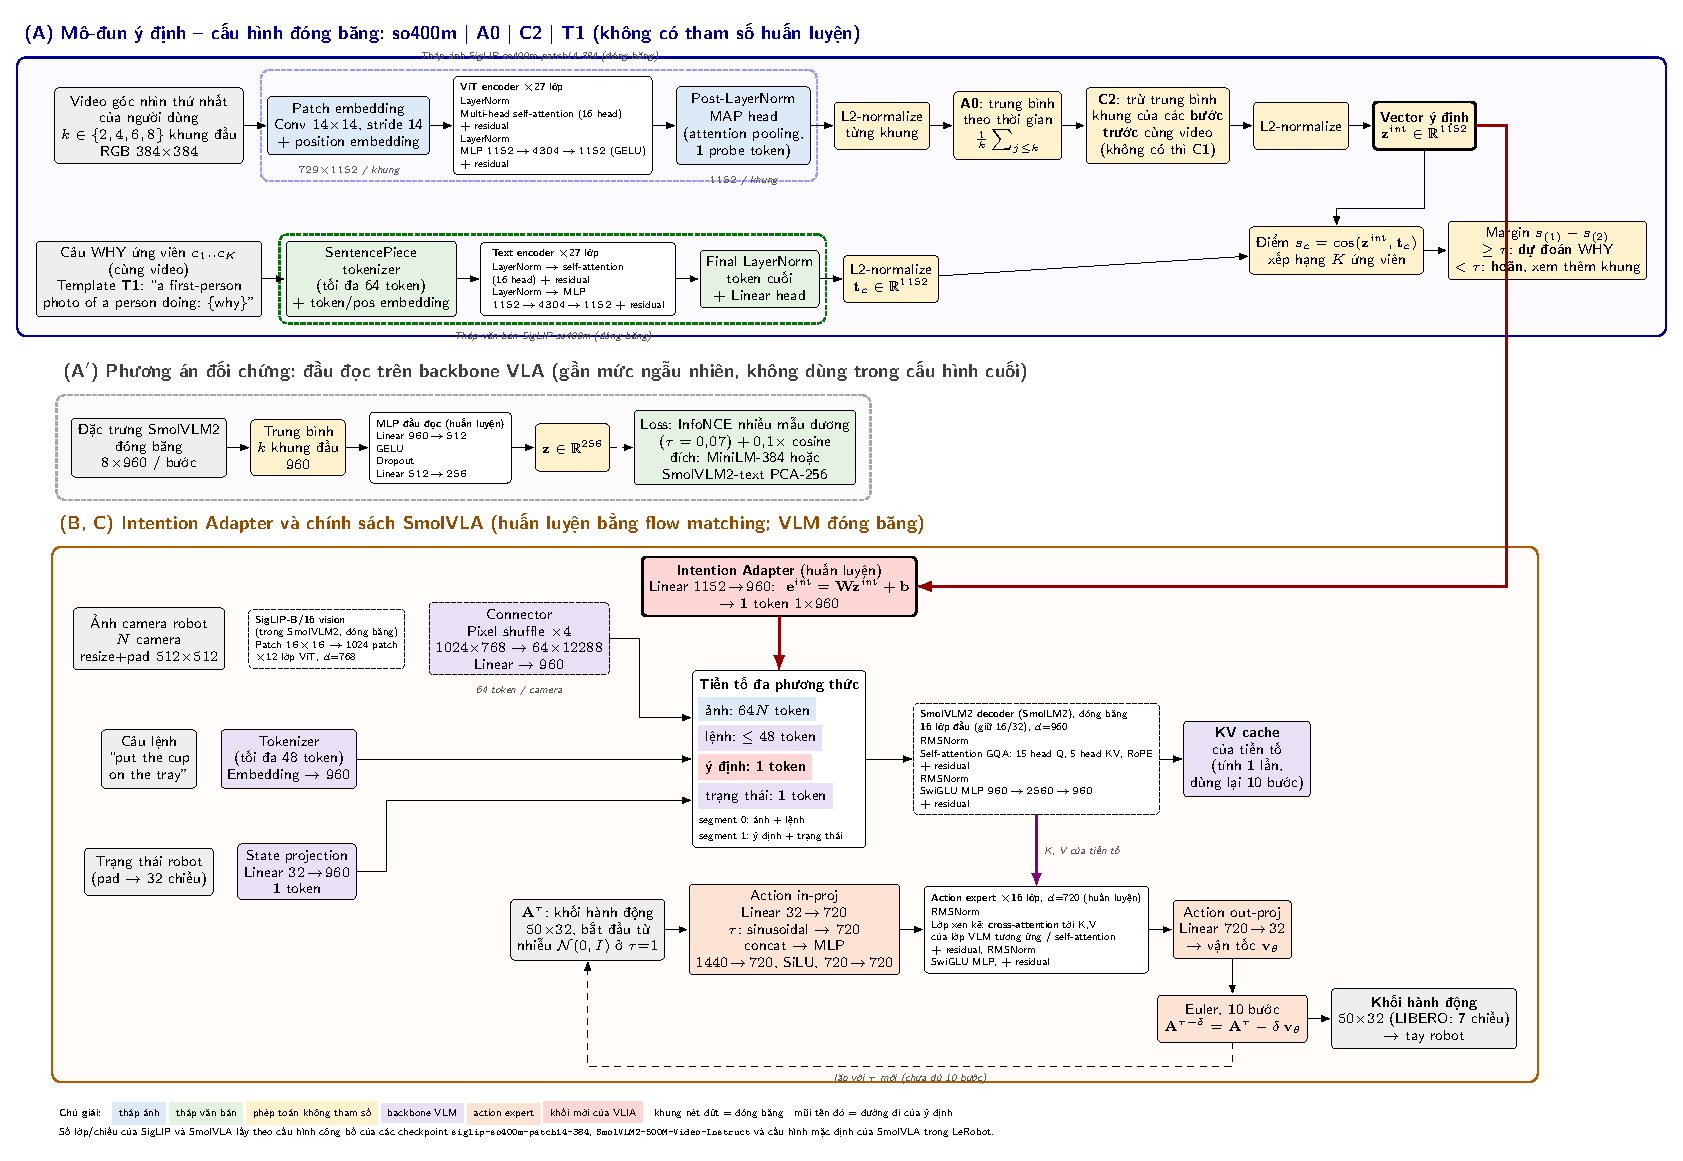
\includegraphics[width=\linewidth]{figs/vlia_detailed.pdf}
\caption{Sơ đồ chi tiết hệ thống VLIA. Đường đi của thông tin ý định tô đỏ; khối viền nét đứt được đóng băng. Số lớp và số chiều bên trong SigLIP, SmolVLM2 và action expert lấy theo cấu hình công bố của các checkpoint.}
\label{fig:vlia_detailed}
\end{figure}

\subsection{Chèn token ý định vào tiền tố}

Token $\mathbf{e}^{\mathrm{int}}$ được chèn vào tiền tố đa phương thức ngay trước token trạng thái robot:
\begin{equation}
  P_{\mathrm{VLIA}} = \big[\,E_{\text{ảnh}};\ E_{\text{lệnh}};\ \mathbf{e}^{\mathrm{int}};\ E_{\text{trạng thái}}\,\big].
\end{equation}
Tiền tố dài thêm đúng một token. Vì tiền tố chỉ được tính một lần và lưu trong bộ nhớ đệm khóa--giá trị (KV cache) trước các bước flow matching, token ý định không làm tăng đáng kể chi phí sinh hành động. Khi tắt cờ ý định, mô hình quay về đúng SmolVLA gốc. Thiết kế này cho phép so sánh công bằng ``có ý định'' và ``không có ý định'' trên cùng chính sách trong các thí nghiệm sau này.

\section{Công cụ quan sát vùng tương tác tay--vật}
\label{sec:hoi_tool}

Để kiểm tra trực quan dữ liệu và kết quả, đồ án xây dựng một công cụ hiển thị ngoại tuyến. Công cụ phát hiện bàn tay trong từng khung bằng MediaPipe Hands \citep{zhang2020mediapipe}, vẽ khung bao bàn tay và một vùng tương tác tay--vật (HOI) ước lượng quanh tay, hiển thị nhãn WHAT/WHY và điểm số của các câu ứng viên (\cref{fig:example}). Vùng HOI ở đây là một hình chữ nhật hình học quanh bàn tay, không phải kết quả của bộ phát hiện vật thể. Dự định ban đầu là thử dùng vùng HOI làm đầu vào cho mô-đun ý định, nhưng phương án này chỉ được thực hiện nếu bàn tay được phát hiện đủ thường xuyên (\cref{sec:hoi_result}).

% =====================================================================
\chapter{Dữ liệu và thiết lập thực nghiệm}
\label{chap:setup}
% =====================================================================

\section{Bộ dữ liệu EgoIntent}

EgoIntent \citep{egointent2026} được xây dựng từ video Ego4D \citep{grauman2022ego4d}. Mỗi video là một hoạt động (ví dụ nhào bột, sửa xe đạp, hái quả) được chia thành các bước thao tác ngắn, mỗi bước kết thúc \textit{trước} khi kết cục xảy ra và có nhãn WHAT, WHY và NEXT. \Cref{fig:example} minh họa một bước thao tác.

\begin{figure}[ht]
\centering
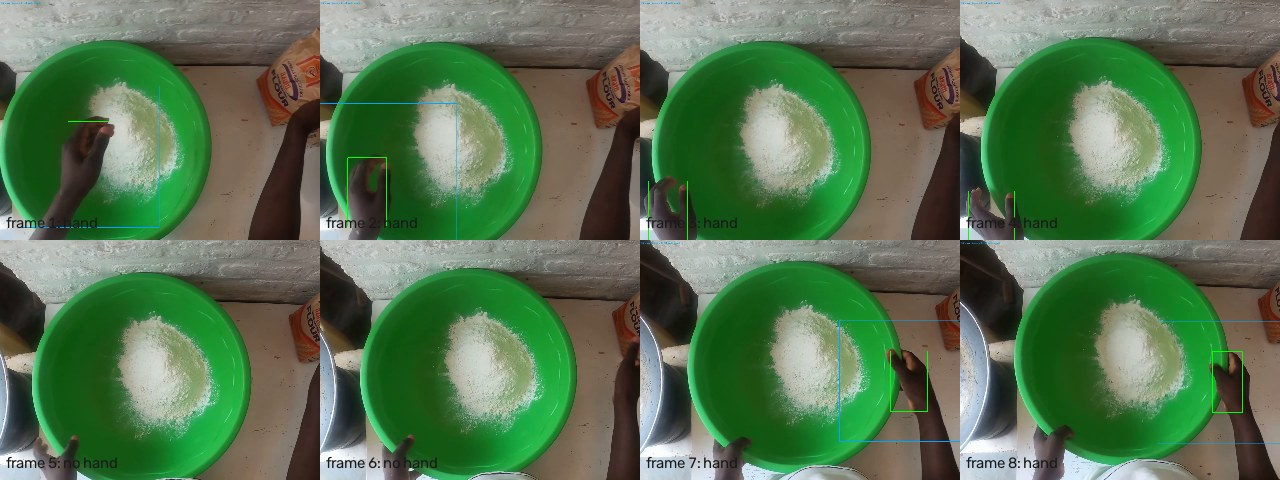
\includegraphics[width=\linewidth]{figs/egointent_example.jpg}
\caption{Tám khung hình của một bước thao tác trong EgoIntent (bối cảnh bếp, hoạt động nhào bột). Nhãn WHAT: ``grasping basin''; nhãn WHY: ``positioning basin''. Khung xanh lá là bàn tay do MediaPipe phát hiện, khung xanh dương là vùng HOI ước lượng; các khung 5 và 6 không phát hiện được tay. Ảnh do công cụ hiển thị của đồ án tạo ra.}
\label{fig:example}
\end{figure}

Đồ án dùng phần huấn luyện và kiểm định của bản đầy đủ, tổng cộng 2.503 bước thao tác (\cref{tab:data}). Phần kiểm thử của bộ dữ liệu được khóa lại và chỉ được dùng một lần cho thí nghiệm ở \cref{sec:fixed_split}.

\begin{table}[ht]
\centering
\caption{Thống kê dữ liệu dùng trong đánh giá chính (phần train + val của EgoIntent).}
\label{tab:data}
\begin{tabular}{lr}
\toprule
Thuộc tính & Giá trị \\
\midrule
Số bước thao tác (mẫu) & 2.503 \\
Số video nguồn & 27 \\
Số bối cảnh (scene) & 13 \\
Số câu WHY khác nhau & 2.032 \\
Số câu WHAT khác nhau & 2.144 \\
Số mẫu mỗi video & 19 -- 125 \\
Số khung lấy đều mỗi mẫu & 8 \\
\bottomrule
\end{tabular}
\end{table}

Các bối cảnh gồm: xưởng mộc, bếp, gara, trang trại, phòng khách, phòng ngủ, xưởng vẽ, tủ quần áo, hiên nhà, hành lang, phòng giặt, sân và không gian ngoài trời. Gần như mọi câu WHY là duy nhất, nên mô hình không thể học thuộc một danh sách nhãn cố định mà phải so khớp ngữ nghĩa giữa video và câu.

\section{Đánh giá chéo theo bối cảnh}
\label{sec:cv}

Một mô hình đoán ý định cho robot phải dùng được ở nơi nó chưa từng thấy. Vì vậy, đồ án chia dữ liệu theo \textit{bối cảnh} thay vì theo mẫu:
\begin{itemize}
  \item 13 bối cảnh được chia thành 8 fold sao cho số mẫu các fold gần bằng nhau. Mỗi video chỉ thuộc một fold.
  \item Với mỗi fold, mô hình được huấn luyện trên 7 fold còn lại và kiểm tra trên fold đó. Như vậy mỗi mẫu được đánh giá đúng một lần, trên bối cảnh mô hình chưa thấy.
  \item Số epoch được chọn trên khoảng 15\% bối cảnh tách ra từ tập huấn luyện của fold, sau đó mô hình được huấn luyện lại trên toàn bộ tập huấn luyện với số epoch đó.
\end{itemize}
So với một tập kiểm định cố định chỉ có 4 video, cách chia này dùng toàn bộ 27 video để đánh giá và tránh việc chọn mô hình trên chính tập dùng để báo cáo.

\section{Tập ứng viên và mức ngẫu nhiên}

\textbf{Xếp hạng toàn tập.} Với mỗi mẫu, tập ứng viên là toàn bộ câu WHY trong fold kiểm tra. Các mẫu có cùng câu WHY đều được tính là đúng. Mức ngẫu nhiên của MRR, Top-1 và Top-3 được tính chính xác theo kích thước fold và số đáp án đúng của từng mẫu; trung bình MRR ngẫu nhiên là 0,0298.

\textbf{Chọn-1-trong-$K$.} Với $K=5$ và $K=10$, mỗi truy vấn có $K-1$ câu nhiễu lấy ngẫu nhiên từ \textit{cùng video}, khác câu đúng. Bộ câu nhiễu được cố định bằng hạt giống tính từ mã mẫu, nên giống hệt nhau giữa các phương án, các độ dài tiền tố và các seed. Cả 2.503 truy vấn đều có đủ ứng viên.

\section{Luật quyết định chốt trước}
\label{sec:prereg}

Khi thử nhiều cấu hình trên dữ liệu nhỏ, rất dễ vô tình chọn cấu hình đẹp nhất rồi báo cáo như phát hiện. Để tránh điều này, các luật sau được ghi vào kho mã \textit{trước} khi chạy thí nghiệm tương ứng và không thay đổi sau khi thấy số liệu:

\begin{description}[leftmargin=0.9cm,style=nextline]
  \item[R1] Đầu đọc (phương án 1) được coi là \textit{trên mức ngẫu nhiên} nếu cận dưới khoảng tin cậy 95\% của lift lớn hơn 1.
  \item[R2] Biểu diễn \texttt{sentence} chỉ được chọn thay cho \texttt{smolvlm\_pca} nếu cận dưới khoảng tin cậy của hiệu ghép cặp lớn hơn 0 ở ít nhất 2/4 độ dài tiền tố.
  \item[G1] Phương án SigLIP \textit{đạt} nếu, ở mọi độ dài tiền tố: cận dưới CI của lift MRR $>1$, cận dưới CI của lift chọn-1-trong-5 $>1$, \textbf{và} độ chính xác chọn-1-trong-5 $\geq 0{,}30$.
  \item[Cổng HOI] Nhánh dùng vùng HOI chỉ được đánh giá nếu tỉ lệ khung phát hiện được bàn tay $\geq 60\%$ trên toàn bộ dữ liệu \textbf{và} $\geq 30\%$ ở mọi bối cảnh.
  \item[N1] Lựa chọn lồng nhau \textit{có ích} nếu hiệu ghép cặp so với phương án 2 có cận dưới CI $>0$ cho \textbf{cả} MRR \textbf{và} chọn-1-trong-5 ở ít nhất 2/4 độ dài tiền tố.
  \item[N2] Lựa chọn lồng nhau \textit{đạt ngưỡng thực dụng} nếu độ chính xác chọn-1-trong-5 $\geq 0{,}30$ và cận dưới CI của lift MRR và lift chọn-1-trong-5 $>1$, ở ít nhất 2/4 độ dài. G1 vẫn giữ nguyên kết quả cũ; N2 là ngưỡng mới, không phải chấm lại G1.
  \item[T1] Trên tập kiểm thử khóa, cấu hình đóng băng \textit{trên mức ngẫu nhiên} nếu cận dưới CI của lift chọn-1-trong-5 $>1$ ở ít nhất 3/4 độ dài.
  \item[T2] Trên tập kiểm thử khóa, cấu hình đóng băng \textit{hơn phương án 2} nếu cận dưới CI của hiệu ghép cặp chọn-1-trong-5 $>0$ ở ít nhất 2/4 độ dài.
  \item[S1b] Dự đoán hay hoãn \textit{có ích} nếu cận dưới CI của (độ chính xác ở độ phủ 50\% $-$ độ chính xác ở độ phủ 100\%) $>0$ ở ít nhất 2/4 độ dài.
  \item[L1, L2] Trên LIBERO: L1 \textit{thông tin mục tiêu quan trọng} nếu cận dưới CI của (thành công với lệnh đúng $-$ với lệnh rỗng) $>0$; L2 \textit{mục tiêu sai còn hại hơn không có mục tiêu} nếu cận dưới CI của (lệnh rỗng $-$ lệnh sai) $>0$.
\end{description}
Hai thí nghiệm phụ cũng có luật chốt trước và đều \textbf{không đạt}: quyết định sớm theo độ chênh (S2) và hiệu chỉnh bằng $k$ láng giềng gần nhất trong không gian câu (K1). Chúng được tóm tắt ở \cref{sec:negative}.

\section{Tập kiểm thử khóa}
\label{sec:locked}

Ngoài đánh giá chéo, đồ án còn một phép thử độc lập trên phần kiểm thử của EgoIntent cho đầu đọc phương án 1. Một video của phần này từng xuất hiện trong tập kiểm định thử nghiệm ban đầu nên bị loại trước khi khóa giao thức, còn lại 407 mẫu từ 4 video, 2 bối cảnh. Giao thức (mô hình, epoch, độ đo) được khóa trước, và tập này chỉ được chạy một lần. Lưu ý rằng tập kiểm thử này tách theo video nhưng không tách theo bối cảnh.

Cấu hình đóng băng của phương án 3 được kiểm tra trên đúng 407 mẫu này theo một quy trình riêng, cũng chỉ chạy một lần:
\begin{itemize}
  \item Tệp \texttt{FROZEN.json} (bộ mã hóa, cách gộp, hiệu chỉnh, mẫu câu, vector trung bình C1 tính trên 2.503 mẫu train + val) và luật T1/T2 được ghi vào kho mã, kèm mã băm, \textit{trước} khi chạy.
  \item Mã đánh giá được kiểm thử trên dữ liệu giả, và từ chối chạy nếu thư mục kết quả đã tồn tại. Lần chạy thật chỉ được thực hiện khi người làm đồ án tự tạo một tệp xác nhận.
  \item C2 trên tập kiểm thử chỉ dùng các bước trước đó của \textit{chính video kiểm thử}, không bao giờ dùng khung của train/val.
  \item Vì chỉ có 4 video, mọi khoảng tin cậy chỉ dựa trên 4 cụm bootstrap và được ghi nhãn là \textit{thăm dò}.
\end{itemize}

\section{Thí nghiệm thông tin mục tiêu trên LIBERO}
\label{sec:libero_setup}

Để biết SmolVLA phụ thuộc vào thông tin mục tiêu đến mức nào, đồ án dùng checkpoint SmolVLA đã huấn luyện lại trên LIBERO-10 (hành động 7 chiều, 1 camera rỗng, 25.000 bước) và chạy 10 tác vụ $\times$ 10 lượt trong ba điều kiện: \textbf{lệnh đúng}; \textbf{lệnh rỗng}; \textbf{lệnh sai}, tức câu lệnh của tác vụ khác theo hoán vị cố định $t\mapsto(t+5)\bmod 10$. Lượt thứ $e$ của mỗi tác vụ dùng cùng trạng thái khởi tạo và cùng hạt giống ở cả ba điều kiện; chỉ chuỗi câu lệnh thay đổi. Khoảng tin cậy dùng bootstrap ghép cặp trên 100 cặp (tác vụ, lượt) và khoảng Wilson 95\% cho từng điều kiện.

\section{Tập dữ liệu tự thu}
\label{sec:own_data}

Để có tình huống nhập nhằng sát với robot cộng tác hơn EgoIntent, đồ án thiết kế một tập dữ liệu nhỏ theo kịch bản ``trà chiều cùng robot'': sáu cảnh (mời robot vào bàn, chọn cốc, chia bánh, sắp xếp bàn, đổi ý giữa chừng, dọn dẹp). Mỗi lần quay, người thực hiện bốc thăm một thẻ mục tiêu bí mật; các mục tiêu khác nhau mở đầu bằng cùng một động tác, và mục tiêu không được nói ra trước khi tay bắt đầu di chuyển. Mỗi video có nhãn \texttt{observation\_end} (thời điểm kết thúc phần được quan sát) và \texttt{outcome\_start} (thời điểm kết cục bắt đầu, sau \texttt{observation\_end} ít nhất 0,5 giây), cùng nhãn WHAT/WHY. Một công cụ kiểm tra tự động từ chối các nhãn vi phạm quy tắc thời gian này.

\TODO{Số người tham gia, số video đã quay, số mục tiêu mỗi cảnh, và kết quả định tính nếu có. Nếu chưa có kết quả, giữ mục này như mô tả giao thức và chuyển sang Hướng phát triển.}

\section{Cài đặt}

Mã nguồn viết bằng Python và PyTorch, dựa trên thư viện LeRobot \citep{cadene2026lerobot} và Hugging Face Transformers. Đặc trưng khung hình được trích xuất một lần và lưu đệm. Thí nghiệm chạy trên một máy trạm Dell Precision 3680 với một GPU NVIDIA. \TODO{Tên GPU và dung lượng bộ nhớ.} Toàn bộ mã, cấu hình và tệp kết quả của các bảng trong đồ án nằm trong kho mã của đề tài\footnote{\url{https://github.com/sgdfgnhmjnfd/vlia-uet}}; các bảng được sinh tự động từ tệp kết quả, không nhập tay.

% =====================================================================
\chapter{Kết quả và thảo luận}
\label{chap:results}
% =====================================================================

Chương này trả lời lần lượt năm câu hỏi nghiên cứu. Mọi số liệu được lấy từ các tệp kết quả trong kho mã. Trong các bảng, ``$\pm$'' là độ lệch chuẩn giữa 3 seed, còn khoảng trong ngoặc vuông là khoảng tin cậy 95\% bootstrap theo video.

\section{Đầu đọc trên tập chia cố định và tập kiểm thử khóa}
\label{sec:fixed_split}

Trước khi chuyển sang đánh giá chéo, đầu đọc phương án 1 (biểu diễn đích \texttt{smolvlm\_pca}) được đánh giá theo cách chia gốc của bộ dữ liệu: huấn luyện trên 2.091 mẫu (23 video), chọn epoch trên tập kiểm định 412 mẫu (4 video), sau đó chạy một lần trên tập kiểm thử khóa (\cref{tab:fixed}).

\begin{table}[ht]
\centering
\caption{Đầu đọc phương án 1 trên tập kiểm định cố định và tập kiểm thử khóa (MRR, trung bình $\pm$ độ lệch chuẩn qua 3 seed).}
\label{tab:fixed}
\begin{tabular}{ccccc}
\toprule
& \multicolumn{2}{c}{Kiểm định (412 mẫu, 4 video)} & \multicolumn{2}{c}{Kiểm thử khóa (407 mẫu, 4 video)} \\
\cmidrule(lr){2-3}\cmidrule(lr){4-5}
Số khung $k$ & MRR & Top-1 & MRR & Top-1 \\
\midrule
2 & 0,0440 $\pm$ 0,0064 & 0,0162 & 0,0290 $\pm$ 0,0028 & 0,0057 \\
4 & 0,0448 $\pm$ 0,0072 & 0,0162 & 0,0288 $\pm$ 0,0033 & 0,0082 \\
6 & 0,0474 $\pm$ 0,0010 & 0,0218 & 0,0294 $\pm$ 0,0045 & 0,0090 \\
8 & 0,0429 $\pm$ 0,0053 & 0,0146 & 0,0314 $\pm$ 0,0035 & 0,0098 \\
\midrule
Mức ngẫu nhiên & 0,0249 & 0,0047 & 0,0318 & 0,0071 \\
\bottomrule
\end{tabular}
\end{table}

Trên tập kiểm định, MRR cao hơn mức ngẫu nhiên khoảng 1,7--1,9 lần, nhưng con số này lạc quan vì epoch được chọn trên chính tập đó. Trên tập kiểm thử khóa, MRR cao nhất (0,0314 ở 8 khung) xấp xỉ mức ngẫu nhiên 0,0318. Nói cách khác, \textbf{đầu đọc không cho thấy khả năng khái quát sang video mới}. Kết quả này là lý do đồ án chuyển sang đánh giá chéo theo bối cảnh (dùng được nhiều video hơn để đánh giá) và thử phương án 2.

\section{RQ1: Đầu đọc trên đặc trưng SmolVLM2 với đánh giá chéo}
\label{sec:rq1}

\Cref{tab:cv} cho kết quả đánh giá chéo theo bối cảnh của phương án 1 với hai cách biểu diễn câu đích.

\begin{table}[ht]
\centering
\caption{Phương án 1 (đầu đọc huấn luyện trên đặc trưng SmolVLM2 đóng băng), đánh giá chéo 8 fold theo bối cảnh, 2.503 mẫu. Mức ngẫu nhiên: MRR 0,0298; chọn-1-trong-5 là 0,20.}
\label{tab:cv}
\small
\begin{tabular}{llcccc}
\toprule
Biểu diễn đích & $k$ & MRR & Lift MRR [CI 95\%] & Chọn 1/5 & Lift 1/5 [CI 95\%] \\
\midrule
\multirow{4}{*}{\texttt{sentence}}
 & 2 & 0,0335 & 1,13 [0,86; 1,43] & 0,216 & 1,08 [1,00; 1,16] \\
 & 4 & 0,0345 & 1,16 [0,88; 1,48] & 0,215 & 1,07 [1,00; 1,16] \\
 & 6 & 0,0353 & 1,18 [0,90; 1,52] & 0,212 & 1,06 [0,98; 1,16] \\
 & 8 & 0,0347 & 1,17 [0,87; 1,51] & 0,219 & 1,10 [1,01; 1,20] \\
\midrule
\multirow{4}{*}{\texttt{smolvlm\_pca}}
 & 2 & 0,0340 & 1,14 [0,95; 1,36] & 0,219 & 1,09 [1,02; 1,17] \\
 & 4 & 0,0338 & 1,14 [0,94; 1,35] & 0,222 & 1,11 [1,03; 1,19] \\
 & 6 & 0,0346 & 1,16 [0,95; 1,39] & 0,223 & 1,12 [1,04; 1,20] \\
 & 8 & 0,0354 & 1,19 [0,98; 1,42] & 0,230 & 1,15 [1,07; 1,23] \\
\bottomrule
\end{tabular}
\end{table}

\begin{ketqua}[Trả lời RQ1]
Đầu đọc huấn luyện trên đặc trưng SmolVLM2 chỉ nhỉnh hơn ngẫu nhiên rất ít. Theo luật R1, lift MRR \textbf{không} vượt ngẫu nhiên ở độ dài tiền tố nào (cận dưới CI luôn $<1$) với cả hai biểu diễn đích. Ở bài toán chọn-1-trong-5, \texttt{smolvlm\_pca} có cận dưới CI $>1$ ở cả 4 độ dài, nhưng độ chính xác chỉ 21,9--23,0\% so với 20\% của đoán mò. Theo luật R2, không có căn cứ để chọn \texttt{sentence} thay cho \texttt{smolvlm\_pca} (hiệu ghép cặp có cận dưới CI $>0$ ở 0/4 độ dài).
\end{ketqua}

Kết quả cũng không đồng đều giữa các video: với \texttt{sentence}, có 8--12 trên 27 video có lift MRR dưới 1 tùy độ dài tiền tố. Điều này cho thấy tín hiệu yếu không đến từ vài video ``khó'' riêng lẻ mà phổ biến trên toàn bộ dữ liệu.

\textbf{Backbone tự chấm điểm.} Một cách khác để dùng backbone mà không huấn luyện là để chính SmolVLM2 đọc khung hình và chấm xác suất của từng câu WHY ứng viên (so với khi không có ảnh). Sau khi sửa lỗi cài đặt của lần chạy đầu, cách này đạt 23,5\% ($k=2$) và 24,6\% ($k=8$) ở chọn-1-trong-5, lift 1,18--1,23 với cận dưới CI trên 1, nhưng thấp hơn SigLIP base khoảng 4,2 điểm (CI không chứa 0). Phép thử đổi video cho CI chứa mức ngẫu nhiên. Như vậy backbone của VLA \textit{có} chứa một chút tín hiệu về mục đích, nhưng yếu hơn rõ so với một bộ mã hóa đã căn chỉnh ảnh--văn bản.

\section{RQ2: Căn chỉnh ảnh--văn bản zero-shot}
\label{sec:rq2}

\Cref{tab:siglip} cho kết quả của SigLIP zero-shot trên đúng cùng fold, cùng tập ứng viên.

\begin{table}[ht]
\centering
\caption{Phương án 2 (SigLIP zero-shot, không huấn luyện) trên cùng 8 fold theo bối cảnh, 2.503 mẫu.}
\label{tab:siglip}
\small
\begin{tabular}{cccccc}
\toprule
$k$ & MRR & Lift MRR [CI 95\%] & Chọn 1/5 & Lift 1/5 [CI 95\%] & Chọn 1/10 \\
\midrule
2 & 0,0671 & 2,25 [1,87; 2,75] & 0,277 & 1,39 [1,23; 1,56] & 0,157 \\
4 & 0,0715 & 2,40 [2,02; 2,88] & 0,275 & 1,38 [1,22; 1,55] & 0,161 \\
6 & 0,0734 & 2,47 [2,06; 2,97] & 0,281 & 1,40 [1,24; 1,58] & 0,167 \\
8 & 0,0765 & 2,57 [2,13; 3,14] & 0,289 & 1,44 [1,27; 1,62] & 0,177 \\
\bottomrule
\end{tabular}
\end{table}

\Cref{fig:lift} đặt hai phương án cạnh nhau. Lift MRR của SigLIP khoảng gấp đôi đầu đọc ở mọi độ dài tiền tố, và các khoảng tin cậy của hai phương án không chồng lên nhau.

\begin{figure}[ht]
\centering
\begin{tikzpicture}
\begin{axis}[
  width=0.82\linewidth,height=6.2cm,
  xlabel={Số khung hình quan sát $k$},
  ylabel={Lift MRR (1 = ngẫu nhiên)},
  xtick={2,4,6,8},
  ymin=0.7,ymax=3.3,
  legend style={font=\footnotesize,draw=none,fill=none,at={(0.5,1.02)},anchor=south,legend columns=3,/tikz/every even column/.append style={column sep=8pt}},
  grid=major,grid style={gray!20},
  every axis plot/.append style={thick,mark size=2pt}]
\addplot[blue!70!black,mark=*,error bars/.cd,y dir=both,y explicit] coordinates {
  (2,2.254) += (0,0.494) -= (0,0.389)
  (4,2.403) += (0,0.475) -= (0,0.387)
  (6,2.466) += (0,0.503) -= (0,0.404)
  (8,2.571) += (0,0.565) -= (0,0.446)};
\addplot[orange!80!black,mark=square*,error bars/.cd,y dir=both,y explicit] coordinates {
  (2,1.14) += (0,0.22) -= (0,0.19)
  (4,1.14) += (0,0.21) -= (0,0.20)
  (6,1.16) += (0,0.23) -= (0,0.21)
  (8,1.19) += (0,0.23) -= (0,0.21)};
\addplot[green!45!black,mark=triangle*,dashed] coordinates {(2,1.13) (4,1.16) (6,1.18) (8,1.17)};
\addplot[gray,dashed,thin,domain=1.5:8.5,samples=2,forget plot] {1};
\legend{SigLIP zero-shot,Đầu đọc (\texttt{smolvlm\_pca}),Đầu đọc (\texttt{sentence})}
\end{axis}
\end{tikzpicture}
\caption{Lift MRR theo số khung quan sát. Thanh sai số là khoảng tin cậy 95\% bootstrap theo video (vẽ cho SigLIP và \texttt{smolvlm\_pca}). Đường nét đứt xám là mức ngẫu nhiên.}
\label{fig:lift}
\end{figure}

\begin{ketqua}[Trả lời RQ2]
Có. Không huấn luyện tham số nào, SigLIP đạt lift MRR 2,25--2,57 với cận dưới CI từ 1,87 trở lên, và độ chính xác chọn-1-trong-5 là 27,5--28,9\%. Tuy vậy, theo luật G1 đã chốt trước, phương án này \textbf{không đạt}: hai điều kiện về khoảng tin cậy thỏa mãn ở 4/4 độ dài, nhưng điều kiện độ chính xác chọn-1-trong-5 $\geq 30\%$ thỏa mãn ở 0/4 độ dài.
\end{ketqua}

Kết quả cho thấy nút thắt của phương án 1 nằm ở \textit{mối liên hệ giữa ảnh và ngôn ngữ}, không phải ở bản thân thông tin thị giác: hai nghìn mẫu không đủ để một đầu đọc học lại mối liên hệ mà SigLIP đã có sẵn từ dữ liệu quy mô Internet. Đây là cơ sở để đồ án chuyển sang các bộ mã hóa đã căn chỉnh, và tìm cách cải thiện chúng mà không huấn luyện (\cref{sec:ladder_result}).

\section{RQ2 (tiếp): Chọn cấu hình lồng nhau}
\label{sec:ladder_result}

Ở cả \textbf{8/8} fold ngoài, lựa chọn lồng nhau chọn cùng một cấu hình: \texttt{siglip-so400m-patch14-384}, gộp trung bình (A0), trừ ngữ cảnh các bước trước (C2), mẫu câu T1. Không fold nào có hai cấu hình đồng hạng. \Cref{tab:ladder} so sánh cấu hình này với phương án 2 trên cùng truy vấn.

\begin{table}[ht]
\centering
\caption{Cấu hình chọn lồng nhau (so400m, A0, C2, T1) so với phương án 2 (SigLIP base, không hiệu chỉnh), 2.503 mẫu, đánh giá ngoài fold. Hiệu là ghép cặp trên cùng truy vấn, CI 95\% bootstrap theo video.}
\label{tab:ladder}
\small
\begin{tabular}{ccccccc}
\toprule
& \multicolumn{3}{c}{Chọn-1-trong-5} & \multicolumn{3}{c}{MRR} \\
\cmidrule(lr){2-4}\cmidrule(lr){5-7}
$k$ & PA 2 & Lồng nhau & Hiệu [CI 95\%] & PA 2 & Lồng nhau & Hiệu [CI 95\%] \\
\midrule
2 & 0,277 & \textbf{0,341} & $+0{,}064$ [$+0{,}039$; $+0{,}089$] & 0,0671 & 0,0747 & $+0{,}0076$ [$-0{,}0037$; $+0{,}0195$] \\
4 & 0,275 & \textbf{0,349} & $+0{,}074$ [$+0{,}049$; $+0{,}100$] & 0,0715 & 0,0777 & $+0{,}0062$ [$-0{,}0059$; $+0{,}0183$] \\
6 & 0,281 & \textbf{0,362} & $+0{,}082$ [$+0{,}051$; $+0{,}112$] & 0,0734 & 0,0825 & $+0{,}0091$ [$-0{,}0024$; $+0{,}0206$] \\
8 & 0,289 & \textbf{0,387} & $+0{,}099$ [$+0{,}062$; $+0{,}134$] & 0,0765 & 0,0850 & $+0{,}0085$ [$-0{,}0026$; $+0{,}0195$] \\
\bottomrule
\end{tabular}
\end{table}

\begin{ketqua}[Kết quả lựa chọn lồng nhau]
\textbf{N2 đạt}: độ chính xác chọn-1-trong-5 là 34,1--38,7\%, vượt 30\% ở 4/4 độ dài; lift MRR 2,51--2,86 và lift chọn-1-trong-5 1,70--1,94, mọi cận dưới CI đều trên 1. \textbf{N1 không đạt}: hiệu chọn-1-trong-5 có cận dưới CI $>0$ ở 4/4 độ dài, nhưng hiệu MRR có CI chứa 0 ở cả 4 độ dài, trong khi luật đòi cả hai.
\end{ketqua}

Hai kiểm tra phụ củng cố kết quả. Thứ nhất, khi thay khung hình bằng khung của một video khác ở bối cảnh khác (313 truy vấn, $k=8$), độ chính xác của cấu hình chọn rơi từ 39,6\% xuống 18,8\%, tức xấp xỉ ngẫu nhiên: tín hiệu đến từ chính nội dung hình ảnh. Thứ hai, trong lưới mô tả (không hiệu chỉnh cho việc chọn), 6 cấu hình đứng đầu đều dùng so400m với C2; bỏ C2 khỏi so400m thì còn 31,1--33,0\%, và thêm C2 cho SigLIP base thì được 29,1--32,1\%. Như vậy cả bộ mã hóa lớn hơn lẫn bước trừ ngữ cảnh đều đóng góp.

\section{RQ2 (tiếp): Tập kiểm thử khóa cho cấu hình đóng băng}
\label{sec:locked_result}

Cấu hình trên được đóng băng và chạy \textbf{một lần duy nhất} trên tập kiểm thử khóa vào ngày 23/10/2026 (\cref{tab:locked}).

\begin{table}[ht]
\centering
\caption{Tập kiểm thử khóa (407 mẫu, 4 video), chạy một lần. Mức ngẫu nhiên: chọn-1-trong-5 là 0,20, MRR 0,0318. CI 95\% bootstrap trên 4 video (thăm dò).}
\label{tab:locked}
\small
\begin{tabular}{cccccc}
\toprule
& \multicolumn{2}{c}{Chọn-1-trong-5} & & \multicolumn{2}{c}{MRR} \\
\cmidrule(lr){2-3}\cmidrule(lr){5-6}
$k$ & Đóng băng [lift CI] & PA 2 & Hiệu [CI 95\%] & Đóng băng & PA 2 \\
\midrule
2 & 0,219 [1,04; 1,14] & 0,204 & $+0{,}015$ [$-0{,}010$; $+0{,}038$] & 0,0459 & 0,0631 \\
4 & 0,246 [1,16; 1,30] & 0,211 & $+0{,}034$ [$+0{,}013$; $+0{,}048$] & 0,0488 & 0,0594 \\
6 & 0,278 [1,20; 1,62] & 0,224 & $+0{,}054$ [$+0{,}010$; $+0{,}097$] & 0,0557 & 0,0660 \\
8 & \textbf{0,302} [1,29; 1,73] & 0,214 & $+0{,}089$ [$+0{,}044$; $+0{,}148$] & 0,0615 & 0,0653 \\
\bottomrule
\end{tabular}
\end{table}

\begin{ketqua}[Kết quả tập kiểm thử khóa]
\textbf{T1 đạt}: cận dưới CI của lift chọn-1-trong-5 lớn hơn 1 ở 4/4 độ dài. \textbf{T2 đạt}: cấu hình đóng băng hơn phương án 2 với cận dưới CI $>0$ ở 3/4 độ dài ($k=4,6,8$). Ở chọn-1-trong-10, cấu hình đóng băng cũng hơn phương án 2 ở 4/4 độ dài.
\end{ketqua}

Ba điểm cần đọc kèm. (i) Độ chính xác trên tập kiểm thử (21,9--30,2\%) thấp hơn rõ so với đánh giá chéo (34,1--38,7\%); chỉ ở $k=8$ mới chạm 30\%. Phương án 2 cũng giảm (từ 27,5--28,9\% xuống 20,4--22,4\%), nên tập kiểm thử có vẻ khó hơn, nhưng với 4 video thì không tách được hai nguyên nhân. (ii) \textbf{MRR trên toàn tập của cấu hình đóng băng lại thấp hơn phương án 2} ở cả 4 độ dài, với CI nằm dưới 0 ở $k=2$. C2 giúp phân biệt các bước trong cùng video (đúng thứ mà chọn-1-trong-$K$ đo), nhưng không giúp xếp hạng giữa mọi câu WHY của nhiều video. (iii) Phép thử đổi video ($k=8$, 51 truy vấn) cho 31,4\% với khung thật và 21,6\% với khung của video khác, cùng chiều với đánh giá chéo.

Kết quả trên tập kiểm thử vì vậy ủng hộ \textit{có giới hạn} cho cấu hình đề xuất: tín hiệu giữ được trên video mới, ưu thế so với phương án 2 trong bài toán sát với robot vẫn còn, nhưng độ lớn nhỏ hơn và chỉ dựa trên 4 video.

\section{RQ3: Ảnh hưởng của lượng quan sát}
\label{sec:rq3}

Câu hỏi ``quan sát thêm có giúp ích không'' được trả lời bằng hiệu ghép cặp trên cùng các mẫu (\cref{tab:paired}).

\begin{table}[ht]
\centering
\caption{Hiệu ghép cặp khi tăng số khung quan sát (sau trừ trước), cùng 2.503 mẫu, CI 95\% bootstrap theo video.}
\label{tab:paired}
\small
\begin{tabular}{lcc}
\toprule
Phương án, độ đo & $2\to 8$ khung & $6\to 8$ khung \\
\midrule
SigLIP, MRR & $+0{,}0094$ [$+0{,}0053$; $+0{,}0141$] & $+0{,}0031$ [$+0{,}0002$; $+0{,}0060$] \\
SigLIP, chọn 1/5 & $+0{,}0112$ [$+0{,}0014$; $+0{,}0211$] & $+0{,}0076$ [$0{,}0000$; $+0{,}0156$] \\
Đầu đọc \texttt{sentence}, MRR & $+0{,}0012$ [$-0{,}0014$; $+0{,}0039$] & $-0{,}0006$ [$-0{,}0021$; $+0{,}0010$] \\
Đầu đọc \texttt{smolvlm\_pca}, MRR & $+0{,}0014$ [$-0{,}0016$; $+0{,}0043$] & $+0{,}0008$ [$-0{,}0010$; $+0{,}0027$] \\
Đầu đọc \texttt{smolvlm\_pca}, chọn 1/5 & $+0{,}0109$ [$+0{,}0023$; $+0{,}0198$] & $+0{,}0064$ [$-0{,}0023$; $+0{,}0151$] \\
\bottomrule
\end{tabular}
\end{table}

\begin{ketqua}[Trả lời RQ3]
Với SigLIP, MRR tăng đều khi quan sát thêm: từ 2 lên 8 khung tăng $+0{,}0094$ (khoảng 14\% tương đối) và khoảng tin cậy không chứa 0. Với đầu đọc, hiệu MRR nhỏ và mọi khoảng tin cậy đều chứa 0, tức không phát hiện được lợi ích của việc quan sát thêm. Như vậy chỉ khi biểu diễn đã căn chỉnh tốt, thêm bằng chứng thị giác mới chuyển thành khả năng phân định mục tiêu tốt hơn.
\end{ketqua}

Mức tăng này vẫn nhỏ so với khoảng cách tới một hệ thống dùng được: ở 8 khung, câu đúng chỉ đứng đầu trong 28,9\% số lần chọn-1-trong-5 với SigLIP base, và 38,7\% với cấu hình chọn lồng nhau. Điều này phù hợp với bản chất của bài toán, vì nhiều bước thao tác kết thúc trước khi mục đích lộ rõ.

\section{RQ5: Dự đoán hay hoãn}
\label{sec:rq5}

\Cref{tab:selective} cho kết quả khi mô-đun ý định (cấu hình chọn lồng nhau) chỉ trả lời các truy vấn có độ chênh cao nhất.

\begin{table}[ht]
\centering
\caption{Độ chính xác chọn-1-trong-5 theo độ phủ, dùng độ chênh top-1 $-$ top-2 làm điểm tin cậy (2.503 mẫu, ngoài fold). CI 95\% bootstrap theo video.}
\label{tab:selective}
\small
\begin{tabular}{cccccc}
\toprule
$k$ & Phủ 100\% & Phủ 50\% & Phủ 20\% & Lợi ích ở 50\% [CI 95\%] & AURC (ngẫu nhiên) \\
\midrule
2 & 0,341 & 0,410 & 0,533 & $+0{,}069$ [$+0{,}039$; $+0{,}096$] & 0,549 (0,659) \\
4 & 0,349 & 0,418 & 0,557 & $+0{,}069$ [$+0{,}045$; $+0{,}095$] & 0,534 (0,651) \\
6 & 0,362 & 0,441 & 0,577 & $+0{,}079$ [$+0{,}053$; $+0{,}106$] & 0,517 (0,638) \\
8 & 0,387 & 0,457 & 0,609 & $+0{,}070$ [$+0{,}040$; $+0{,}097$] & 0,497 (0,613) \\
\bottomrule
\end{tabular}
\end{table}

\begin{ketqua}[Trả lời RQ5]
Có. \textbf{S1b đạt} ở 4/4 độ dài: chỉ trả lời 50\% truy vấn chắc nhất thì độ chính xác tăng 6,9--7,9 điểm; chỉ trả lời 20\% thì đạt 53--61\%. Với ngưỡng tính từ các fold khác (không rò rỉ), độ phủ thực tế khớp mục tiêu (0,50 và 0,20), độ chính xác lần lượt là 40,7--46,1\% và 53,3--60,9\%, đều cao hơn khi trả lời mọi truy vấn. Ở độ phủ 80\% thì lợi ích không còn rõ.
\end{ketqua}

Với cấu hình SigLIP base, cùng phép thử chỉ cho lợi ích +2,6 đến +3,5 điểm (S1, đạt nhưng nhỏ). Điểm tin cậy vì vậy hữu ích hơn hẳn khi bộ mã hóa tốt hơn. Cần lưu ý độ chênh chỉ là một điểm quyết định đơn giản, chưa phải thước đo đã kiểm chứng cho việc ``đã đủ bằng chứng hay chưa'', và kết quả này chưa được kiểm tra trên tập kiểm thử khóa.

\section{Các hướng đã thử và không đạt}
\label{sec:negative}

\begin{itemize}
  \item \textbf{Quyết định sớm theo độ chênh (S2, không đạt).} Robot dừng quan sát ở khung đầu tiên có độ chênh vượt ngưỡng. So với dùng số khung cố định có cùng số khung trung bình, độ chính xác chỉ hơn có ý nghĩa ở 1/4 mức ngân sách ($+0{,}014$ ở 5 khung), không đạt yêu cầu 2/4.
  \item \textbf{Hiệu chỉnh bằng láng giềng gần nhất (K1, không đạt).} Lấy 20 truy vấn huấn luyện giống nhất rồi pha câu WHY của chúng vào điểm số làm MRR \textit{giảm} 0,004--0,007 (CI dưới 0 ở 3/4 độ dài) và không cải thiện chọn-1-trong-5. Cấu hình đóng băng vì vậy dùng trọng số kNN bằng 0.
\end{itemize}

\section{Phân tích lỗi}
\label{sec:errors}

\subsection{Giới hạn do câu đồng nghĩa}

Các câu WHY được viết tự do, nên cùng một video thường có những câu gần nghĩa nhau. Theo bộ mã hóa câu all-MiniLM-L6-v2, 66,6\% truy vấn có ít nhất một câu WHY khác trong cùng video với cosine $\geq 0{,}8$, và 44,5\% có câu với cosine $\geq 0{,}9$. Vì đánh giá chỉ coi câu trùng khớp chính xác là đúng, các câu đồng nghĩa bị tính là sai, làm điểm số tuyệt đối bị chặn trên. Hai chẩn đoán phụ đã được chốt trước để ước lượng ảnh hưởng này. Thứ nhất, khi chỉ lấy câu nhiễu có cosine $<0{,}8$ với câu đúng và với nhau (bài toán chọn-1-trong-5 ``sạch''), độ chính xác của SigLIP ở 8 khung tăng từ 28,9\% lên 30,8\%. Thứ hai, khi coi các câu có cosine $\geq 0{,}9$ với câu đúng cũng là đúng, MRR tăng lên 0,112 với lift 2,13 [1,71; 2,66]. Các con số này chỉ là chẩn đoán và \textbf{không} được dùng để đổi kết luận G1.

\subsection{Một ví dụ thất bại}

Với bước thao tác ở \cref{fig:example} (nhãn WHY ``positioning basin''), SigLIP ở 8 khung xếp các ứng viên theo thứ tự: ``prepare to knead dough'' (cosine 0,101), ``developing dough consistency'' (0,085), ``forming cohesive dough'' (0,072), ``cleaning the table surface'' (0,056), và câu đúng ``positioning basin'' đứng cuối (0,020). Mô hình nhận ra đúng \textit{hoạt động chung} (nhào bột), nhưng không phân biệt được \textit{bước} cụ thể trong hoạt động đó. Đây là kiểu lỗi đặc trưng của bài toán: các ứng viên cùng video chia sẻ đồ vật và bối cảnh, chỉ khác nhau ở mục đích của bước.

\subsection{Lỗi cùng tác vụ}

Trên tập kiểm thử khóa, khi đầu đọc chọn sai ở Top-1, 46--53\% số lỗi là chọn nhầm sang một câu WHY \textit{của cùng hoạt động}. Con số này cần đọc kèm mức ngẫu nhiên tương ứng, vì tỉ lệ ứng viên cùng hoạt động trong tập xếp hạng khác nhau giữa các tập chia.

\section{Cổng phát hiện bàn tay}
\label{sec:hoi_result}

MediaPipe phát hiện được bàn tay trong 58,2\% khung hình (11.652/20.024). Tỉ lệ rất khác nhau giữa các bối cảnh (\cref{tab:hoi}): cao ở tủ quần áo (88,8\%) và hành lang (84,5\%), nhưng rất thấp ở hiên nhà (10,3\%), phòng giặt (15,3\%), sân (15,9\%) và không gian ngoài trời (24,8\%).

\begin{table}[ht]
\centering
\caption{Tỉ lệ khung hình phát hiện được bàn tay theo bối cảnh (MediaPipe Hands).}
\label{tab:hoi}
\small
\begin{tabular}{lr@{\hspace{1.5cm}}lr}
\toprule
Bối cảnh & Tỉ lệ & Bối cảnh & Tỉ lệ \\
\midrule
Tủ quần áo & 88,8\% & Gara & 61,8\% \\
Hành lang & 84,5\% & Xưởng vẽ & 61,8\% \\
Xưởng mộc & 76,2\% & Trang trại & 32,2\% \\
Bếp & 71,6\% & Không gian ngoài trời & 24,8\% \\
Phòng ngủ & 67,2\% & Sân & 15,9\% \\
Phòng khách & 61,9\% & Phòng giặt & 15,3\% \\
& & Hiên nhà & 10,3\% \\
\midrule
\multicolumn{2}{l}{\textbf{Toàn bộ}: 58,2\%} & \multicolumn{2}{l}{Cổng yêu cầu: $\geq 60\%$ và mỗi bối cảnh $\geq 30\%$} \\
\bottomrule
\end{tabular}
\end{table}

Cổng HOI \textbf{không đạt} ở cả hai điều kiện, nên theo luật đã chốt, nhánh dùng vùng HOI không được đánh giá. Đồ án vì vậy \textbf{không có kết luận} về việc tập trung vào vùng tay--vật có giúp mô-đun ý định hay không. Công cụ hiển thị vẫn được giữ để quan sát dữ liệu.

\section{RQ4: Tích hợp vào SmolVLA}
\label{sec:rq4}

\Cref{tab:integration} liệt kê các kiểm thử cài đặt cho Intention Adapter và đường chèn token ý định trong SmolVLA.

\begin{table}[ht]
\centering
\caption{Kiểm thử cài đặt phần tích hợp ý định vào SmolVLA.}
\label{tab:integration}
\small
\begin{tabularx}{\linewidth}{l X c}
\toprule
Thành phần & Nội dung kiểm tra & Kết quả \\
\midrule
Intention Adapter & Gradient truyền ngược được qua adapter & Đạt \\
Chèn tiền tố & Độ dài tiền tố tăng đúng 1 token & Đạt \\
Vị trí token & Token ý định nằm ngay trước token trạng thái & Đạt \\
KV cache & Token ý định có mặt trong bộ nhớ đệm khi suy luận & Đạt \\
Hàm mất mát & Mất mát flow matching hữu hạn; forward/backward nhất quán & Đạt \\
Tắt ý định & Mô hình quay về đúng SmolVLA gốc khi tắt cờ & Đạt \\
Lưu/tải & Lưu và tải lại checkpoint không mất trọng số & Đạt \\
\bottomrule
\end{tabularx}
\end{table}

Toàn bộ kiểm thử được chạy lại với ba kích thước vector ý định $d\in\{256, 768, 1152\}$, ứng với phương án 1, phương án 2 và cấu hình đóng băng (so400m), trên một SmolVLA khởi tạo ngẫu nhiên có cùng kiến trúc với checkpoint LIBERO. Cả 7 kiểm thử đạt ở cả 3 kích thước: tiền tố dài từ 77 lên 78 token, khóa trong KV cache cũng dài 78 và thay đổi khi đổi $\mathbf{z}^{\mathrm{int}}$, sai khác tối đa khi tắt cờ và khi lưu/tải đều bằng 0. Đây chỉ là bằng chứng cài đặt đúng, không phải kết quả khoa học.

\subsection{SmolVLA phụ thuộc vào thông tin mục tiêu đến mức nào}

Đồ án huấn luyện lại SmolVLA \textit{không có ý định} trên LIBERO-10 \citep{liu2023libero} với cấu hình hành động 7 chiều đúng chuẩn; lần đánh giá tham chiếu đạt 24\% trên 100 lượt. Hai lượt huấn luyện trước đó bị loại vì cấu hình sai (hành động 6 chiều, thiếu camera rỗng). Với checkpoint này, thí nghiệm ở \cref{sec:libero_setup} cho kết quả ở \cref{tab:libero}.

\begin{table}[ht]
\centering
\caption{SmolVLA trên LIBERO-10 với ba loại câu lệnh, cùng trạng thái khởi tạo và hạt giống (10 tác vụ $\times$ 10 lượt mỗi điều kiện).}
\label{tab:libero}
\small
\begin{tabular}{lccc}
\toprule
Câu lệnh & Thành công & Tỉ lệ & Wilson 95\% \\
\midrule
Đúng & 19/100 & 0,19 & [0,125; 0,278] \\
Rỗng & 0/100 & 0,00 & [0,000; 0,037] \\
Sai (lệnh của tác vụ khác) & 0/100 & 0,00 & [0,000; 0,037] \\
\bottomrule
\end{tabular}
\end{table}

Theo tác vụ, số lượt thành công với lệnh đúng là 0, 1, 3, 7, 1, 3, 3, 0, 0, 1 trên 10. Mọi lượt với lệnh rỗng hoặc sai đều chạy hết giới hạn 520 bước mà không hoàn thành. \textbf{L1 đạt}: lệnh đúng hơn lệnh rỗng $+0{,}19$ [$+0{,}12$; $+0{,}27$]. \textbf{L2 không đạt}: cả hai điều kiện đều bằng 0, nên không thể thấy lệnh sai có hại hơn lệnh rỗng hay không. Tỉ lệ 19\% dùng tập khởi tạo khác với lần đánh giá 24\% nên hai số không được so sánh với nhau.

\begin{giaithich}[Thí nghiệm này nói gì và không nói gì]
Thí nghiệm cho thấy SmolVLA \textit{hoàn toàn} dựa vào câu lệnh để biết phải làm gì: không có mục tiêu thì robot không làm xong việc nào. Đây là lý do một robot cộng tác cần nguồn thông tin mục tiêu khác khi người không nói ra. Tuy nhiên, câu lệnh rỗng và sai nằm ngoài phân bố huấn luyện, nên thí nghiệm chỉ đo sự phụ thuộc vào kênh ngôn ngữ; nó \textbf{chưa} cho thấy token ý định dự đoán sẽ giúp được.
\end{giaithich}

\begin{ketqua}[Trả lời RQ4]
Có, ở mức cài đặt: thông tin ý định đi vào SmolVLA đúng vị trí, có gradient, và không phá vỡ mô hình gốc khi tắt, với cả ba kích thước vector. SmolVLA phụ thuộc gần như tuyệt đối vào thông tin mục tiêu (19\% so với 0\%). Đồ án \textbf{chưa} đo việc token ý định dự đoán có thay thế hay bổ sung được cho câu lệnh hay không.
\end{ketqua}

\section{Thảo luận chung}

\textbf{Điều gì đã được chứng minh.} Trên bối cảnh chưa thấy, một bộ mã hóa ảnh--văn bản đã căn chỉnh sẵn phân định mục tiêu tốt gấp khoảng hai lần đầu đọc được huấn luyện trên đặc trưng của backbone VLA, và hưởng lợi từ việc quan sát thêm. Một bộ mã hóa lớn hơn cùng bước trừ ngữ cảnh các bước trước đưa độ chính xác chọn-1-trong-5 lên 34--39\%, được chọn ổn định ở 8/8 fold, và giữ được ưu thế so với cấu hình gốc trên tập kiểm thử khóa chạy một lần. Điểm tin cậy cho phép robot biết khi nào nên chờ. Về phía robot, SmolVLA không làm được việc gì khi thiếu thông tin mục tiêu.

\textbf{Điều gì chưa được chứng minh.} Trên tập kiểm thử, độ chính xác chỉ 22--30\%, thấp hơn rõ so với đánh giá chéo, và MRR toàn tập còn kém cấu hình gốc. Mọi kết luận trên tập kiểm thử chỉ dựa trên 4 video. Tác động của token ý định dự đoán lên hành vi robot chưa được đo. Dữ liệu chính chỉ có 27 video, 13 bối cảnh.

\textbf{Ý nghĩa cho thiết kế VLIA.} Kết quả gợi ý rằng mô-đun ý định nên dựa trên biểu diễn đã căn chỉnh ảnh--ngôn ngữ, tập trung vào \textit{phần thay đổi} so với ngữ cảnh trước đó, và đi kèm cơ chế hoãn khi chưa chắc. Việc huấn luyện thêm (nếu có) nên ở dạng nhẹ trên biểu diễn đó thay vì học từ đầu trên dữ liệu nhỏ.

% =====================================================================
\chapter{Kết luận và hướng phát triển}
\label{chap:conclusion}
% =====================================================================

\section{Kết luận}

Đồ án nghiên cứu cách tăng cường khả năng hiểu ý định người dùng cho robot cộng tác dựa trên mô hình VLA. Các kết quả chính:
\begin{enumerate}
  \item Đề xuất kiến trúc VLIA, bổ sung cho SmolVLA một mô-đun ý định tách rời và một token ý định trong tiền tố đa phương thức; phần tích hợp vượt qua bộ kiểm thử cài đặt.
  \item Xây dựng quy trình đánh giá mô-đun ý định qua bài toán phân định sớm mục tiêu, với đánh giá chéo theo bối cảnh, ứng viên nhiễu cùng video, mức ngẫu nhiên chính xác, bootstrap theo video và luật quyết định chốt trước.
  \item Chỉ ra rằng đầu đọc huấn luyện trên đặc trưng đóng băng của SmolVLM2 gần như ngang ngẫu nhiên (lift MRR 1,13--1,19, CI chứa 1; ngang ngẫu nhiên trên tập kiểm thử khóa).
  \item Chỉ ra rằng SigLIP zero-shot tăng lift MRR lên 2,25--2,57 (CI hoàn toàn trên 1) và cải thiện khi quan sát thêm khung hình, nhưng chưa đạt ngưỡng G1.
  \item Lựa chọn lồng nhau trên 90 cấu hình không huấn luyện chọn cùng cấu hình so400m + trừ ngữ cảnh ở 8/8 fold, đạt 34,1--38,7\% chọn-1-trong-5 (N2 đạt). Trên tập kiểm thử khóa chạy một lần, cấu hình đóng băng đạt 21,9--30,2\%, trên ngẫu nhiên (T1) và hơn cấu hình gốc (T2).
  \item Cơ chế dự đoán hay hoãn tăng độ chính xác 6,9--7,9 điểm khi trả lời một nửa số truy vấn.
  \item Trên LIBERO-10, SmolVLA thành công 19\% với lệnh đúng và 0\% khi lệnh rỗng hoặc sai.
\end{enumerate}

\section{Hạn chế}

\begin{itemize}
  \item \textbf{Chưa có thí nghiệm hành vi.} Chưa đo việc token ý định cải thiện thao tác của robot, trên mô phỏng hay robot thật (UR5).
  \item \textbf{Dữ liệu nhỏ.} 27 video, 13 bối cảnh; khoảng tin cậy theo video chỉ mô tả tập này.
  \item \textbf{Đánh giá theo câu trùng khớp.} Câu đồng nghĩa bị tính là sai, làm điểm tuyệt đối bị chặn trên.
  \item \textbf{Tập kiểm thử nhỏ.} Tập kiểm thử khóa chỉ có 4 video, 2 bối cảnh, tách theo video nhưng không tách theo bối cảnh; khoảng tin cậy trên đó chỉ mang tính thăm dò. Tập này đã được dùng một lần và không được chạy lại.
  \item \textbf{Lựa chọn trên dữ liệu đánh giá chéo.} Cấu hình chọn lồng nhau được chọn trên các fold huấn luyện của cùng 27 video, và kết quả dự đoán hay hoãn chưa được kiểm tra trên tập kiểm thử.
  \item \textbf{Lưu trữ đặc trưng.} Đặc trưng SigLIP lưu ở dạng float16; khi tái tạo, độ chính xác chọn-1-trong-5 lệch 1 truy vấn trên 2.503 ở $k=2$ và $k=4$.
  \item \textbf{Thí nghiệm LIBERO.} Một checkpoint, một seed huấn luyện, 10 lượt mỗi tác vụ; lệnh rỗng và sai nằm ngoài phân bố huấn luyện.
\end{itemize}

\section{Hướng phát triển}

\begin{itemize}
  \item Huấn luyện SmolVLA có token ý định trên LIBERO và so sánh với lệnh rỗng: token ý định có lấy lại được một phần trong 19 điểm mất đi khi thiếu câu lệnh không.
  \item Ablation riêng cho bước trừ ngữ cảnh (C2) với luật chốt trước, và so sánh với một VLM lớn chấm điểm zero-shot (ví dụ Qwen2.5-VL-7B).
  \item Thu thêm dữ liệu kiểm thử tách theo bối cảnh để có khoảng tin cậy đáng tin hơn 4 video.
  \item Hoàn thiện tập dữ liệu tự thu theo kịch bản trà chiều và đánh giá trên robot UR5.
\end{itemize}

% =====================================================================
% TÀI LIỆU THAM KHẢO
% =====================================================================
\cleardoublepage
\addcontentsline{toc}{chapter}{Tài liệu tham khảo}
\begin{thebibliography}{99}
\small

\bibitem{brohan2022rt1}
A.~Brohan \emph{et al.}, ``RT-1: Robotics Transformer for real-world control at scale,'' \emph{arXiv:2212.06817}, 2022.

\bibitem{zitkovich2023rt2}
B.~Zitkovich \emph{et al.}, ``RT-2: Vision-language-action models transfer web knowledge to robotic control,'' in \emph{Proc. Conference on Robot Learning (CoRL)}, PMLR 229, 2023, pp.~2165--2183.

\bibitem{openx2024}
Open X-Embodiment Collaboration, ``Open X-Embodiment: Robotic learning datasets and RT-X models,'' in \emph{Proc. IEEE Int. Conf. Robotics and Automation (ICRA)}, 2024, pp.~6892--6903.

\bibitem{shukor2025smolvla}
M.~Shukor \emph{et al.}, ``SmolVLA: A vision-language-action model for affordable and efficient robotics,'' \emph{arXiv:2506.01844}, 2025.

\bibitem{cadene2026lerobot}
R.~Cadene \emph{et al.}, ``LeRobot: An open-source library for end-to-end robot learning,'' in \emph{Proc. Int. Conf. Learning Representations (ICLR)}, 2026.

\bibitem{lipman2023flow}
Y.~Lipman, R.~T.~Q. Chen, H.~Ben-Hamu, M.~Nickel, and M.~Le, ``Flow matching for generative modeling,'' in \emph{Proc. ICLR}, 2023.

\bibitem{marafioti2025smolvlm}
A.~Marafioti \emph{et al.}, ``SmolVLM: Redefining small and efficient multimodal models,'' \emph{arXiv:2504.05299}, 2025.

\bibitem{huggingface2025smolvlm2}
O.~Zohar, M.~Farre, A.~Marafioti \emph{et al.}, ``SmolVLM2: Bringing video understanding to every device,'' Hugging Face technical blog, 2025.

\bibitem{liu2023libero}
B.~Liu, Y.~Zhu, C.~Gao, Y.~Feng, Q.~Liu, Y.~Zhu, and P.~Stone, ``LIBERO: Benchmarking knowledge transfer for lifelong robot learning,'' in \emph{Advances in Neural Information Processing Systems (NeurIPS)}, 2023.

\bibitem{grauman2022ego4d}
K.~Grauman \emph{et al.}, ``Ego4D: Around the world in 3,000 hours of egocentric video,'' in \emph{Proc. IEEE/CVF CVPR}, 2022, pp.~18995--19012.

\bibitem{grauman2024egoexo4d}
K.~Grauman \emph{et al.}, ``Ego-Exo4D: Understanding skilled human activity from first- and third-person perspectives,'' in \emph{Proc. IEEE/CVF CVPR}, 2024, pp.~19383--19400.

\bibitem{egointent2026}
``EgoIntent: An open-ended benchmark for intent understanding at pre-outcome micro-steps in egocentric procedural activities,'' Hugging Face dataset card (\texttt{py2279105943/EgoIntent}), 2026.

\bibitem{mascaro2023intention}
E.~Valls Mascaro, H.~Ahn, and D.~Lee, ``Intention-conditioned long-term human egocentric action anticipation,'' in \emph{Proc. IEEE/CVF WACV}, 2023, pp.~6048--6057.

\bibitem{zhao2024antgpt}
Q.~Zhao \emph{et al.}, ``AntGPT: Can large language models help long-term action anticipation from videos?'' in \emph{Proc. ICLR}, 2024.

\bibitem{chu2026insight}
Q.~Chu, H.~Zhang, M.~Liu, Y.~Feng, H.~Shi, and L.~Nie, ``Intention-guided cognitive reasoning for egocentric long-term action anticipation,'' in \emph{Proc. AAAI Conf. Artificial Intelligence}, 2026.

\bibitem{radford2021clip}
A.~Radford \emph{et al.}, ``Learning transferable visual models from natural language supervision,'' in \emph{Proc. Int. Conf. Machine Learning (ICML)}, PMLR 139, 2021, pp.~8748--8763.

\bibitem{zhai2023siglip}
X.~Zhai, B.~Mustafa, A.~Kolesnikov, and L.~Beyer, ``Sigmoid loss for language image pre-training,'' in \emph{Proc. IEEE/CVF ICCV}, 2023, pp.~11975--11986.

\bibitem{reimers2019sbert}
N.~Reimers and I.~Gurevych, ``Sentence-BERT: Sentence embeddings using Siamese BERT-networks,'' in \emph{Proc. EMNLP-IJCNLP}, 2019, pp.~3982--3992.

\bibitem{zhang2020mediapipe}
F.~Zhang \emph{et al.}, ``MediaPipe Hands: On-device real-time hand tracking,'' \emph{arXiv:2006.10214}, 2020.

\end{thebibliography}

\end{document}
